
\documentclass[oneside,intlimits,reqno]{scrbook}

\usepackage{array}
\usepackage{enumerate}
\usepackage{mathrsfs}
\usepackage{mathtools}
\usepackage{pgf,tikz}
\usetikzlibrary{arrows}
\usepackage{extarrows}
\usepackage{graphicx,makeidx}
\usepackage{a4wide}
\usepackage{ragged2e}
\usepackage[nottoc]{tocbibind}
\usepackage{amsmath,amssymb,amsthm,amsfonts}
\usepackage{mathabx}
\usepackage[utf8]{inputenc}
\usepackage[czech]{babel}
\usepackage{relsize}



\usepackage[unicode,breaklinks=true,hypertexnames=false]{hyperref}
\def\dotminus{\mathbin{\ooalign{\hss\raise1ex\hbox{.}\hss\cr
			\mathsurround=0pt$-$}}}
		
\usepackage[inline,attach]{asymptote}
\usepackage[dvips]{attachfile2}
%definice textu nad rovnítkem
\newcommand{\equal}[1]{\mathop{\overset{#1}{\resizebox{\widthof{.{\ensuremath{\mathop{\overset{#1}{\mathop{=}}}}.}}}{\heightof{=}}{$\mathop{=}$}}}}

%redefinice znaků
\renewcommand{\epsilon}{\varepsilon}
\let\crossedphi\phi
\renewcommand{\phi}{\varphi}
\renewcommand{\rho}{\varrho}
\renewcommand{\emptyset}{\font\cmsy = cmsy10 at 12pt\hbox{\cmsy \char 59}}


%definice českých uvozovek
\def\bq{\mbox{\kern.1ex\protect\raisebox{-1.3ex}[0pt][0pt]{''}\kern-.1ex}}
\def\eq{\mbox{\kern-.1ex``\kern.1ex}}
\gdef\uv#1{\bq #1\eq}


\renewcommand{\d}{\mathrm{d}} % diferenciál
\newcommand{\me}{\mathrm{e}} % eulerovo číslo
\newcommand{\E}{\mathbb{E}} % střední hodnota
\newcommand{\D}{\mathrm{D}} %  rozptyl
\newcommand{\LL}{\mathscr{L}}
\newcommand{\Loss}{\mathscr{L}}
\newcommand{\FF}{\mathrm{F}} % distribuční funkce
\newcommand{\PP}{\mathbb{P}} % pravděpodobnost
\newcommand{\NN}{\mathcal{N}}
\newcommand{\MSE}{\mathrm{MSE}}
\newcommand{\Exp}{\mathrm{Exp}}
\newcommand{\NF}{\mathrm{F}}
\newcommand{\AN}{\mathcal{AN}}
\newcommand{\sgn}{\mathrm{sgn}}
\newcommand{\A}{\mathrm{A}}

\newcommand{\prostor}{(\Omega,\mathcal{A},\PP)} % prostor
\newcommand{\mi}{\mathrm{i}} % imaginární jednotka
\newcommand{\R}{\mathbb{R}} % množina reálných čísel
\renewcommand{\C}{\mathbb{C}} % množina komplexních čísel
\newcommand{\Z}{\mathbb{Z}} % množina celých čísel
\newcommand{\N}{\mathbb{N}} % množina přirozených čísel
\newcommand{\Cc}{\mathcal{C}} % funkce třídy C (spojité)
\newcommand{\I}{\mathbb{I}} % identita
\newcommand{\Identita}[1]{\mathbb{I}_{#1}} % identita
\newcommand{\fisher}{\mathbb{I}} % Fisherova matice
\newcommand{\RR}{\mathcal{R}}
\newcommand{\Be}{\mathrm{Be}}
\newcommand{\Bi}{\mathrm{Bi}}
\newcommand{\X}{\textbf{X}}
\newcommand{\Q}{\mathbb{Q}}
\newcommand{\bt}{\boldsymbol{\theta}}
\newcommand{\bdelta}{\boldsymbol{\delta}}
\newcommand{\Y}{\textbf{Y}}

\newcommand{\PEX}{\PP^\X}
\newcommand{\fex}{f_\X}
\newcommand{\FEX}{\FF_\X}


\newcommand{\Aa}{\mathcal{A}}
\newcommand{\Bb}{\mathcal{B}}
\renewcommand{\t}{\theta} % theta
\newcommand{\bmu}{\boldsymbol{\mu}} % vektorové mí

\newcommand{\htm}{\widehat{\t}_\txt{M}}
\newcommand{\htb}{\widehat{\t}_\txt{B}}
\newcommand{\html}{\widehat{\t}_\txt{ML}}
\newcommand{\htn}{\widehat{\t}_n}
\newcommand{\rhn}{R_{H_0}}
\newcommand{\Phiast}{\crossedphi^\ast}
\newcommand{\rhno}{\overline{R}_{H_0}}
\newcommand{\freg}{\mathcal{F}_{reg}}
\newcommand{\fregp}{\mathcal{F}_{reg}^+}
\newcommand{\fregml}{\mathcal{F}_{reg}^\txt{ML}}
\newcommand{\fregmle}{\mathcal{F}_{reg}^\txt{MLE}}
\newcommand{\RE}{\mathrm{RE}_{2,1}}
\newcommand{\ARE}{\mathrm{ARE}_{2,1}}


%matematické výrazy
\newcommand{\tg}{\mathop{\mathrm{tg}}}
\newcommand{\argmin}{\mathop{\mathrm{argmin}}}
\newcommand{\argmax}{\mathop{\mathrm{argmax}}}
\newcommand{\argsup}{\mathop{\mathrm{argsup}}}
\renewcommand{\Re}{\mathop{\mathrm{Re}}}
\newcommand{\Ran}{\mathop{\mathrm{Ran}}}
\newcommand{\supp}{\mathop{\mathrm{supp}}}
\renewcommand{\Im}{\mathop{\mathrm{Im}}}
\newcommand{\Cov}{\mathbb{C}\mathrm{ov}}


%konvergence
\newcommand{\sj}{\stackrel{s.j.}{\longrightarrow}}
\newcommand{\Pto}{\stackrel{\PP}{\to}}
\newcommand{\wto}{\stackrel{w}{\to}}
\newcommand{\Dto}{\stackrel{\mathscr{D}}{\to}}
\newcommand{\PSJ}{\stackrel{\PP,s.j.}{\longrightarrow}}
\newcommand{\Lto}{\stackrel{(\mathscr{L})}{\to}}
\newcommand{\sjP}{\stackrel{s.j.~\PP}{\longrightarrow}}
\newcommand{\Lp}{\stackrel{L_p}{\longrightarrow}}

%nadtržítka
\newcommand{\overbar}[1]{\mkern 1mu\overline{\mkern-1mu#1\mkern-3mu}\mkern 3mu}
\newcommand{\Oxn}{\overbar{\rule{0ex}{1.8ex}X_n}}
\newcommand{\Oyn}{\overbar{\rule{0ex}{1.8ex}Y_n}}
\newcommand{\Ox}[1]{\overbar{\rule{0ex}{1.8ex}X_{#1}}}
\newcommand{\Oy}[1]{\overbar{\rule{0ex}{1.8ex}Y_{#1}}}
\newcommand{\oxn}{\overbar{\rule{0ex}{1.33ex}X_n}}
\newcommand{\ox}[1]{\overbar{\rule{0ex}{1.33ex}X_{#1}}}
\newcommand{\oy}[1]{\overbar{\rule{0ex}{1.33ex}Y_{#1}}}
\newcommand{\oyn}{\overbar{\rule{0ex}{1.33ex}Y_n}}
\newcommand{\omn}{\overbar{\rule{0ex}{1.3ex}\mu_n}}
\newcommand{\walpha}{\widehat{\alpha}}
\newcommand{\wbeta}{\widehat{\beta}}
\newcommand{\wgamma}{\widehat{\gamma}}

\newcommand{\hyn}{\widehat{y}_n}
\newcommand{\hyi}{\widehat{y}_i}
\newcommand{\hy}{\widehat{y}}
\newcommand{\lyn}{\overline{y}_n}
\newcommand{\ly}{\overline{y}}
\newcommand{\lhyn}{\overline{\hy}_n}
\newcommand{\lhy}{\overline{\hy}}
\newcommand{\lyi}{\overline{y}_i}
\newcommand{\RMR}{\mathrm{R}}
\newcommand{\SST}{\mathrm{SST}}
\newcommand{\SSE}{\mathrm{SSE}}
\newcommand{\SSR}{\mathrm{SSR}}
\newcommand{\lei}{\overline{e}_i}
\newcommand{\hei}{\widehat{e}_i}
\newcommand{\he}{\widehat{e}}
\newcommand{\Hobv}{\mathcal{H}_\text{obv}}
\newcommand{\HCF}{\mathcal{H}_\mathrm{CF}}
\newcommand{\RF}{\mathcal{R}}

\newcommand{\pB}{\widehat{p}_B}
\newcommand{\pML}{\widehat{p}_\mathrm{ML}}
\newcommand{\wmu}{\widehat{\mu}}

\newcommand{\TV}{\mathrm{TV}}
\newcommand{\Ev}{\mathrm{Ev}}
\newcommand{\Dd}{\mathscr{D}}
\newcommand{\Rr}{\mathscr{R}}

\newcommand{\oxnn}{\overbar{\rule{0ex}{1.33ex}x_n}}

%stříšky
\newcommand{\hsn}{\widehat{\sigma}_n^2}

%posloupnosti
\newcommand{\posl}{(X_j)_{j=1}^{+\infty}}
\newcommand{\poslkon}{(X_j)_{j=1}^{n}}
\newcommand{\posln}{(X_n)_{n=1}^{+\infty}}
\newcommand{\poslnn}{(\X_n)_{n=1}^{+\infty}}

%sumy
\newcommand{\suminftyo}{\sum\limits_{n=0}^{+\infty}}
\newcommand{\suminfty}{\sum\limits_{n=1}^{+\infty}}
\newcommand{\sumainfty}[1]{\sum\limits_{#1}^{+\infty}}
\newcommand{\suminftylo}{\sum\limits_{l=0}^{+\infty}}
\newcommand{\sumin}{\sum\limits_{i=1}^{n}}
\newcommand{\sumjn}{\sum\limits_{j=1}^{n}}
\newcommand{\sm}[2]{\sum\limits_{ #1 }^{ #2 }}


\newcommand{\dom}[1]{\mathop{\mathrm{Dom} (#1)}} % definiční obor
\newcommand{\mat}[1]{\mathbf #1}
\newcommand{\abs}[1]{\left|#1\right|}
\renewcommand{\b}[1]{\left( #1 \right)}
\newcommand{\nor}[1]{\left\|#1\right\|}
\newcommand{\Br}[1]{\Bigl(#1\Bigr)}
\newcommand{\br}[1]{\bigl(#1\bigr)}
\newcommand{\e}[1]{\me^{#1}}
\newcommand{\inv}[1]{#1^{-1}}
\newcommand{\ini}{\theta\in\Theta}
\newcommand{\init}[1]{\theta\in\Theta\subset\R^#1}

\newcommand{\txt}[1]{\mathrm{{\footnotesize  #1 }}}
\newcommand{\matice}[4]{\left(\begin{array}{cc}	#1 & #2 \\ #3 & #4	\end{array} \right)}
\newcommand{\maticehrana}[4]{\left[\begin{array}{cc}	#1 & #2 \\ #3 & #4	\end{array} \right]}
\newcommand{\vektor}[2]{\left(\begin{array}{c}	#1  \\  #2	\end{array} \right)}
\newcommand{\p}[1]{\PP\left( #1 \right)}
\newcommand{\EE}[1]{\E\left[ #1 \right]}
\newcommand{\n}[1]{\NN\left( #1 \right)}
\newcommand{\hypothesis}[2]{H_0: #1 ~\text{vs.}~ H_1: #2 }
\newcommand{\hypothesiswide}[2]{H_0: #1 \qquad\text{vs.}\qquad H_1: #2 }
\newcommand{\silofunkce}[1]{\beta_\crossedphi\big|_{\Theta_{#1}}}
\newcommand{\silofunkceast}[1]{\beta_{\Phiast}\big|_{\Theta_{#1}}}
\newcommand{\hypothesisap}[2]{H'_0: #1 ~\text{vs.}~H'_1: #2 }
\newcommand{\test}[1]{\boxed{\text{TEST: $H_0$ zamítáme, pokud } #1 .}}
\renewcommand{\S}{\mathbb{S}}


% Prostředí
\theoremstyle{definition}
\newtheorem{define}{Definice}[chapter]
\theoremstyle{plain}
\newtheorem{theorem}[define]{Věta}
\newtheorem{lemma}[define]{Lemma}
\newtheorem{dusl}[define]{Důsledek}
\newtheorem{corollary}[define]{Tvrzení}
\renewcommand{\proofname}{Důkaz}

\theoremstyle{remark}
\newtheorem{example}[define]{\textsc{Příklad}}
\newtheorem{remark}[define]{\textsc{Poznámka}}

\renewcommand{\indexname}{Rejstřík}

\frenchspacing

\usepackage[symbol]{footmisc} %Speciálná \footnote{}
\renewcommand{\thefootnote}{\fnsymbol{footnote}}

\hypersetup{
 	pdftitle={01BAPS - Bayesovské principy ve statistice},
 	pdfauthor={WIKI Skripta},
 	pdfsubject={Zápisky z přednášek BAPS, FJFI ČVUT},
 	pdfkeywords={Bayesovské principy ve statistice},
 	bookmarksnumbered=true,
 	colorlinks=true,
 	pdfpagemode={UseOutlines}
 }
\makeindex

\title{01BAPS}
\date{\today}
\author{Václav Kůs, Martin Kovanda \\ opravy Jan Trödler \\ ilustrace Filip Bár}

\begin{document}

% ****************************************************************************************************************************
%                             FRONTMATTER
% ****************************************************************************************************************************
\frontmatter
\maketitle

\newpage
\pdfbookmark[0]{Obsah}{obsah}
\tableofcontents

\chapter*{Předmluva}
\pdfbookmark[0]{Předmluva}{predmluva}

Materiál byl sestaven na~základě poznámek a~prezentací Ing. Václava Kůse, Ph.D. Zmíněné přednášky proběhly v~zimním semestru akademického roku 2020/2021 na~Fakultě jaderné a
fyzikálně inženýrské ČVUT v~Praze. Přednášky nebyly uskutečněny prezenční formou vzhledem k~probíhající pandemii Covid-19. 

Tento učební text je určen posluchačům 1.~ročníku navazujícího magisterského studia navštěvujícím kurs 01BAPS\emph{ Bayesovské principy ve~statistice}, který je zařazen
mezi předměty oboru AMSM. Při~sestavování textu se~předpokládaly znalosti základů matematiky na~úrovni absolvování kurzů 01MAB2-4, 01LAB1-2, 01MIP a~01MAS.



% ****************************************************************************************************************************
%                             MAINMATTER
% ****************************************************************************************************************************
\mainmatter
%%%%%%%%%%%%%%%%% 1. lesson
\chapter{Úvodní motivační úlohy ze~spolehlivosti, medicíny, biologie, ekonometrie, experimentální fyziky.}
Ve statistice provádíme experimenty, abychom získali nějaký užitek, případně abychom mohli předvídat budoucí děje. 

\begin{example}[Požár lesa ve~Španělsku]~
	 \begin{enumerate}[a)]
		\item Abychom mohli předvídat budoucí požáry lesa, musíme si nejprve rozmyslet, jestli jsou požáry náhodné, tedy jestli je daná veličina deterministická, nebo stochastická úloha. 
		\item V~tom případě ale potřebujeme model, který by úlohu popisoval. V~rámci toho modelu musíme zkoumat faktory ovlivňující požáry lesa. Těch je však mnoho, a~proto musíme vybrat ty relevantní. 
		\item Dále potom záleží na~struktuře dat. Vezmeme $p$ jako pravděpodobnost, že v~lese vznikne požár. Potom logistický model pro~tuto pravděpodobnost vypadá jako
		$$ p=\frac{\e{\alpha_1 h+\alpha_2t+\alpha_3x}}{1+\e{\alpha_1 h+\alpha_2 t+\alpha_3 x}}, $$
		kde $h$ je vlhost, $t$ teplota a~$x$ stupeň péče o~les.
		\item Snažíme se~nyní odhadnout parametry $\walpha_1,\walpha_2,\walpha_3$. na~základě dostupných dat.
		\item Dále musíme ověřit tento model na~reálné situaci.
	\end{enumerate} 
\end{example}
\begin{example}[Capture-Recapture] V~rybníce je $N$ ryb. Abychom tento počet zjistili, aniž bychom museli vylovit celý rychník, vylovíme pouze $r$ ryb, označíme je a~pustíme zpět do~vody. Dále počkáme, až budou ryby rovnoměrně rozmístěny a~vylovíme $s$ ryb. Z~nich bude $x$ značit počet označených ryb.
	
Rozdělení $x$ je potom $X\sim f_X(x)=\frac{\binom{r}{x}\binom{N-r}{s-x}}{\binom{N}{s}}\sim\mathrm{Hyp}(N,r,s)$. Nyní nám jde o~to odhadnout, jak vypadá $\widehat{N}$ jako odhad počtu ryb v~rybníce. Po~krátké úvaze dospějeme k~tomu, že $\widehat{N}=\frac{rs}{x}$.
\end{example}
\begin{example}[Analýza dat o~přežití]
	Mějme $X\geq0$ jako čas do~poruchy (ale i~něčeho pozitivního). Pokud tento problém řešíme stochasticky, máme rozdělení $X\sim \FF_X,f_X$ a~hledáme $\EE X=\t$, kterou značíme i~jako MTTF (\textit{mean time to failure}). Zavedeme dále \textbf{intenzitu poruch} jako $r_X(x)=\frac{f_X(x)}{1-\FF_X(x)}$. Úkolem je potom nalézt $\widehat{\t}$.
\end{example}
\begin{example}[MEX] Představme si počítačovou síť, kde máme za~úkol kontrolovat switch. Obecně o~jednotlivých uživatelích sítě nevíme nic (nevíme, že zrovna dneska bude někdo stahovat filmy apod.) Označme $X_i \sim \NN$ jako průtok dat od~$i$-tého uživatele. Potom chceme mít pod~kontrolou pravděpodobnost přetečení switche, tedy $\p{\sumin X_i>C_s}<\e{-\gamma}$ (např. $10^{-10}$, což je velice nepravděpodobné). Zabýváme se~tedy jevy, které se~dějí velice zřídka, ale které by mohli mít i~vážný dopad, např. u~povodní. 
\end{example}
\begin{example}[Ekonometrie]
	Víme, že změna mzdy souvisí se~změnou ceny komodity, tedy $\Delta M \stackrel{?}{\leftrightarrow}\Delta C$ (např. $\Delta C=\alpha+\beta(\Delta M)^2+\gamma\ln\Delta M+\epsilon$). Abychom mohli takový vztah odhadnout, potřebujeme data z~minulosti $\big(\Delta M_i,\Delta C_i\big)_{i=1}^n$. Z~toho pak lze odhadnout $\walpha,\wbeta,\wgamma$. Deterministický přístup by byl použít např. lineární regresi. Pokud však bude součástí zadání předpovědět hodnotu v~místě, které nikdy nebylo k~dispozici, nemůžeme si být jisti výsledkem, viz obr.\ref{fig:overfitting}. Cílem je odhadnout $\epsilon$, což můžeme například pomocí CLT jako $\epsilon=\sumin \epsilon_i\sim\AN$.
\end{example}

\begin{figure}[h]
	\centering
	\begin{tikzpicture}[line cap=round,line join=round,>=triangle 45,x=6.0cm,y=6.0cm]
	\clip(-0.26,-0.05) rectangle (1.5,0.68);
	\draw [color=green!45!black](0.75,0.21) node[anchor=north west] {Přeučení};
	\draw [color=red!65!black](0.12,0.45) node[anchor=north west] {Nedostatečné naučení};
	\draw [color=blue!55!black](0.80,0.34) node[anchor=north west] {Skutečná závislost};
	\draw (0,-0.05) -- (0,0.68);
	\draw [domain=-0.26:1.28] plot(\x,{(-0-0*\x)/1});
	\draw[line width=1pt,color=red!65!black] plot[raw gnuplot, id=func0] function{set samples 10000; set xrange [-0.16:1.18]; plot 0.18*x+0.22};
	\draw[line width=1pt,color=blue!55!black] plot[raw gnuplot, id=func1] function{set samples 10000; set xrange [-0.16:1.18]; plot 1.35*x**2-1.06*x+0.31};
	\draw[line width=1pt,color=green!45!black] plot[raw gnuplot, id=func2] function{set samples 10000; set xrange [-0.16:1.18]; plot 1476.55*x**8-5318.13*x**7+7495.45*x**6-5161.41*x**5+1738.28*x**4-227.24*x**3-4.93*x**2+2.01*x+0.25};
	\begin{scriptsize}
	\fill [color=black] (0.7,0.16) circle (3.0pt);
	\fill [color=black] (0.65,0.13) circle (3.0pt);
	\fill [color=black] (-0.09,0.35) circle (3.0pt);
	\fill [color=black] (0.03,0.3) circle (3.0pt);
	\fill [color=black] (0.14,0.26) circle (3.0pt);
	\fill [color=black] (0.2,0.18) circle (3.0pt);
	\fill [color=black] (0.26,0.17) circle (3.0pt);
	\fill [color=black] (0.98,0.62) circle (3.0pt);
	\fill [color=black] (0.93,0.48) circle (3.0pt);
	\fill [color=black] (0.7,0.16) circle (3.0pt);
	\fill [color=black] (0.65,0.13) circle (3.0pt);
	\fill [color=black] (-0.09,0.35) circle (3.0pt);
	\fill [color=black] (0.03,0.3) circle (3.0pt);
	\fill [color=black] (0.14,0.26) circle (3.0pt);
	\fill [color=black] (0.2,0.18) circle (3.0pt);
	\fill [color=black] (0.26,0.17) circle (3.0pt);
	\fill [color=black] (0.98,0.62) circle (3.0pt);
	\fill [color=black] (0.93,0.48) circle (3.0pt);
	\end{scriptsize}
	\end{tikzpicture}
	\caption{Příklad přeučení a~nedostatečného naučení u~kvadratických dat.}
	\label{fig:overfitting}
\end{figure}


$$ \mathcal{F}=\big\{ f(x,\t):\t\in\Theta\subset\R^k \big\} $$
$X_i~iid~f$, kde $f_\textbf{X}=\prod f_{X_i}$. $\widehat{\t}$ na~základě $\textbf{x}$ (rozhodnutí o~$\t$). Znáhodníme parametr $\t$, kde $\t\sim\pi(\t)$.
\begin{theorem}[Bayesova] 
	Mějme $(H_k)_{k=1}^{n,+\infty}$ jako úplný rozklad $\Omega,~A~\in \Aa , ~\PP(A)>0$. Potom $\forall k\in\N$ platí, že 
	\[
	\PP(H_k|A)=\frac{\PP(A|H_k)\PP(H_k)}{\sum\limits_{j=1}^{n,+\infty}\PP(A|H_j)\PP(H_j)}
	\]
	\begin{proof}
		$$\PP(H_k|A)=\frac{\PP(H_k\cap A)}{\PP(A)}=\frac{\PP(A|H_k)\PP(H_k)}{\sum\limits_{j=1}^{n,+\infty}\PP(A|H_j)\PP(H_j)}$$
	\end{proof}
\end{theorem}
\begin{theorem}
	Mějme $X,Y$ jako náhodné veličiny s~$f_{X,Y}$. Pak
	$$ f(y|x)=\frac{f(x|y)g(y)}{\int_{\mathcal{Y}}f(x|y)g(y)dy}. $$
\begin{proof}
$$ f(y|x)=\frac{f_{X,Y}(x,y)}{f(x)}=\frac{f(x|y)g(y)}{\int_{\mathcal{Y}}f(x|y)g(y)dy} $$
\end{proof}

\end{theorem}
%%%%%%%%%%%%%%%%%%%% 2. lesson
\begin{remark}
	Bayesova věta... znáhodnění $\t$. Máme třídu hustot $\mathcal{F}=\big\{f(x,\t):\t\in\Theta\subset\R^k\big\},~\t\sim\pi(\t)$. Dále $X\sim f(x|\t)\Rightarrow \X=(X_1,...,X_n)~iid~f_\X(\textbf{x}|\t)$.
	
	Z toho vyplývá, že $\phi(\textbf{x},\t)=f(\textbf{x}|\t)\pi(\t)$, $m(\textbf{x})=\int\phi(\textbf{x},\t)\d \t=\int f(\textbf{x}|\t)\pi(\t)\d\t$ jako marginální rozdělení $\X$. 
	$$ \pi(\t|\textbf{x})\stackrel{B}{=}\frac{\phi(\textbf{x},\t)}{m(\textbf{x})}=\frac{f(\textbf{x}|\t)\pi(\t)}{\int_\Theta f(\textbf{x}|\t)..........} $$
	\begin{itemize}
	\item 	$\pi(\t)$ nazýváme \textit{apriorní hustota}
	\item   $\pi(\t|\textbf{x})$ nazýváme \textit{aposteriorní hustota}
	\item znáhodnění $\theta$ je tedy způsob, jak sumarizovat dosažitelnou informaci o $\theta$
	\end{itemize}

	
\end{remark}


$\pi(\t)$ lze určit na základě:\begin{enumerate}[a)]
	\item objektivní informace, tj. znalost z~předchozích úloh (z minulosti),
	\item subjektivní informace (znalost experta, naše znalost, ...),
	\item kombinace a) a~b) ($C=\alpha_1\pi_1(\t)+\alpha_2\pi_2(\t)$), případně více a) nebo více b)
	\item neurčitost (neznalost)
\end{enumerate}

\begin{center}
    
    \begin{tikzpicture}
    \node[inner sep=0pt] (pic) at (0,0)
    {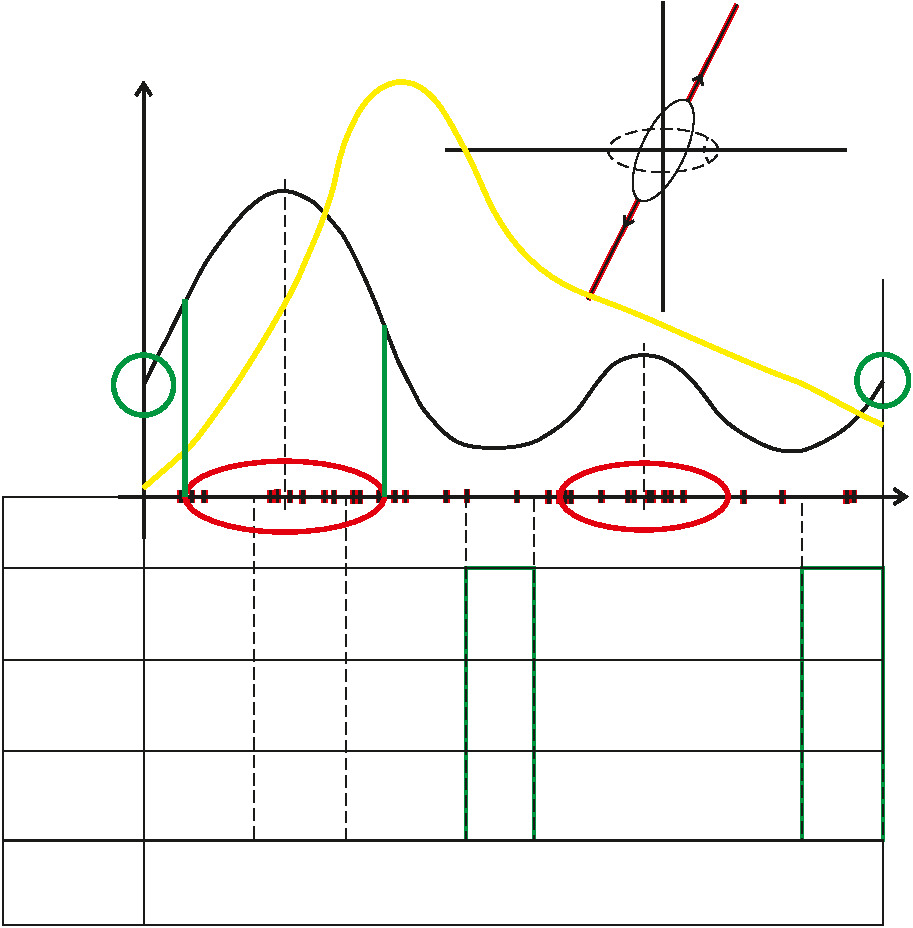
\includegraphics[width=10cm]{pictures/picture_1_3.pdf}};
    \draw [color=red](-3.5,-1.3) node[anchor=north west] {Dodelat popisky? Budeme chtít i tento příklad?};
    \end{tikzpicture}
\end{center}

\begin{remark}
	Tímto způsobem by se~dalo pojmout i~strojové učení. To bere nějaká trénovací a~testovací data, kde na~trénovacích datech dochází k~učení modelu a~na~testovacích datech (která nebyla použita při~trénování) pak vyhodnocuje, jak moc daný model funguje.
\end{remark}
Takto víceméně funguje rozhodování, která děláme. 
$$ \pi(\t)\stackrel{\text{data}}{\longrightarrow}\pi_n(\t|\textbf{x})\to \widehat{\t}_B=\EE{\pi(\t|\textbf{x})}$$
Chtěli bychom, aby byl náš odhad $\widehat{\t}_B\big( \pi_s(\t|\textbf{x}) \big)$ s~rostoucím $n\to+\infty$ stále méně ovlivněn $\pi(\t)$.

\begin{example} --zde by to chtělo asi lepší popis--
	Představme si, že máme biliárový stůl a dva hráče, kteří mezi sebou hrají. První hráč dostane kouli na pozici (1) s pravděpodobností $p$, která leží mezi 0 a 1. Druhý hráč chce poté odhadnout místo, kde se koule prvního hráče nachází, čili chce dostat odhad $\widehat{p}=?$ na základě $n$ šťouchů, o kterých víme, že se buďto dotkly koule, či nikoliv. 
	
	statistika: máme $n$ šťouchů s~rovnoměrným rozdělením. Označme $X$ jako počet neťuků. $X(\omega)=\textbf{x}$, což jsou data, která máme k~dispozici a~ptáme se~na~odhad $\widehat{p}=?$.
	
	-------------PIC03----------------
	
	\begin{enumerate}[a)]
		\item Předpokládejme, že 1. hráč je uniformní. Potom $p\sim\pi(p)=1$ na~$(0,1)$ (podle principu neurčitosti). Potom
		$$ X\sim\Bi(n,p)=f(x|p).$$
		Dále pak 
		$$ \pi(\t|x)=\frac{f\cdot\pi}{\int_0^1 f\pi\d p}=\frac{\binom{n}{x}p^x(1-p)^{n-x}\cdot 1}{\int_0^1 \binom{n}{x}p^x(1-p^{n-x}\cdot1 \d p)}=\mathrm{Beta}(x+1,n-x+1).$$
		Z toho vyplývá, že
		$$ \widehat{\t}_B=\widehat{p}_B=\EE{p|x}=\int...=\frac{x+1}{n+2}.$$
		Potom se~můžeme ptát, jaké je $p$, pokud známe $\textbf{x}$. Klasický odhad by byl ve~tvaru $\widehat{p}_{\mathrm{ML}}=\frac{x}{n}$.
		\item $\pi(\t)=\pi(p)=\mathrm{Beta}(\alpha,\beta)$ Z~toho pak 
		\[
		\begin{split}
		\pi(p|x)&=\frac{f\cdot\pi}{\underbrace{\int f\pi}_c}=\frac{1}{c}\binom{n}{x}p^x(1-p)^n\cdot \frac{1}{B(...)}p^{\alpha-1}(1-p)^{\beta-1}=\frac{1}{c'}p^{x+\alpha-1}(1-p)^{n-x+\beta-1}=\\&=\mathrm{Beta}(x+\alpha,n-x+\beta).
		\end{split}
		\] 
		Dále
		$$ \widehat{p}_B=\EE{\mathrm{Beta}(x+\alpha,n-x+\beta)}=\frac{x+\alpha}{n+\alpha+\beta}\doteq\frac{x}{n} = \widehat{p}_{ML} ~~~\text{pro velká \textit{n}, tedy i velká \textit{x}}$$
	\end{enumerate}
\end{example}

\begin{center}
    
    \begin{tikzpicture}
    \node[inner sep=0pt] (pic) at (0,0)
    {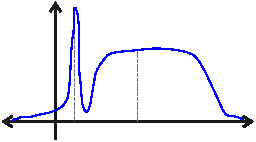
\includegraphics[width=10cm]{pictures/picture_2_1.pdf}};
    \draw [color=black](-2.5,-2) node[anchor=north west] {$ \widehat{\t}_{\text{MLE}} $};
    \draw [color=black](0.2,-2) node[anchor=north west] {$ \widehat{\t}_{\text{B}} $};
    \draw [color=blue](2.8,1.2) node[anchor=north west] {$ \pi(\t|\textbf{x}) $};
    \end{tikzpicture}
\end{center}

$\pi(\t)=c\neq0$ konstantní, takže $\pi(\t)$ můžeme volit tak, aby $\int_\Theta\pi(\t)=+\infty$.
\begin{define}[Nevlastní hustota (apriorní)] Definujeme apriorní nevlastní hustotu jako hustotu $\pi(\theta)$ takovou, že $$ \int\limits_{\Phi}{\pi(\theta)} = +\infty,$$  avšak 
	$$\pi(\t|x)=\frac{f\cdot \pi}{\int f\pi\d\t}$$ je stále regulární hustotou. Nevlastní hustota $\pi(\theta)$ tedy stále nese apriorní informaci o $\theta$.
\end{define}
\begin{example}\begin{enumerate}[a)]
		\item 
	Mějme $X\sim f(x|\mu)=\NN(\mu,1)$, kde $\mu\in\R$. Dále nechť $\pi(\mu)=c\neq0$. Potom$$ \pi(\mu|x)=\frac{f\cdot \pi}{\int_{-\infty}^{+\infty}\frac{1}{\sqrt{2\pi}}\e{-\frac{1}{2}(x-\mu)^2}c\d\mu}=\frac{\e{-\frac{1}{2}(\mu-x)^2}}{\sqrt{2\pi}}\sim\NN(x,1).$$
	Dále pak 
	$$\widehat{\mu}_B=\EE{\NN(x,1)}=x=\widehat{\mu}_{\mathrm{ML}}.$$
	\item Nechť $f=\NN(0,1)$ a~$\pi(\mu)=\NN(0,10)$.
	
	\begin{figure}[h]
	\centering  
    \begin{tikzpicture}
    \node[inner sep=0pt] (pic) at (0,0)
    {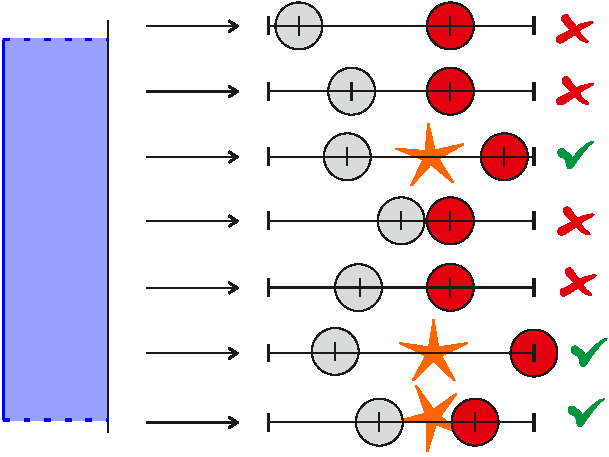
\includegraphics[width=8cm]{pictures/picture_2_2.pdf}};
    \draw [color=blue](-4.0,0.4) node[anchor=north west] {$ \text{U}(0,1) $};
    \draw [color=black](-0.75,3.5) node[anchor=north west] {$ 0 $};
    \draw [color=black](2.65,3.5) node[anchor=north west] {$ 1 $};
    \draw [color=black](1.6,3.5) node[anchor=north west] {$ p $};
    \draw [color=black](4.6,0.4) node[anchor=north west] {$ \text{Bi}(n,p) $};
    \draw [color=black](-1.9,3.2) node[anchor=north west] {$ \text{X}_{1} $};
    \draw [color=black](-1.9,2.35) node[anchor=north west] {$ \text{X}_{2} $};
    \draw [color=black](-1.9,1.5) node[anchor=north west] {$ \text{X}_{3} $};
    \draw [color=black](-1.9,0.65) node[anchor=north west] {$ \text{X}_{4} $};
    \draw [color=black](-1.9,-1.9) node[anchor=north west] {$ \text{X}_{n} $};
    \end{tikzpicture}
	\caption{Kulečníkový stůl.}
\end{figure}
	
	Pojďme nyní udělat apriorní odhad $\mu$, tedy $\widehat{\mu}_{\mathrm{apr.}}=\EE{\NN(0,10)}=0$. $X=x...f_X$. Dále
	$$ \pi(\mu|x)=\frac{1}{c}f\cdot\pi=\frac{1}{c}\e{-\frac{1}{2}(x-\mu)^2}\e{-\frac{1}{20}(\mu-o)^2}=\frac{1}{c}\e{-\frac{11}{20}(\mu-\frac{10}{11}x)^2}$$ s~rozdělením $\NN\left(\frac{10}{11}x,\frac{10}{11}\right)$.
	Pro odhad $\mu$ pak platí, že
	$$\widehat{\mu}_B=\EE{\pi(\mu|x)}=\int\frac{1}{c}\e{-\frac{11}{20}(\mu-\frac{10}{11}x)^2}\d\mu=\frac{10}{11}x.$$ 
	
	HPD (High Posterior Density) region
	
	\begin{center}
    
    \begin{tikzpicture}
    \node[inner sep=0pt] (pic) at (0,0)
    {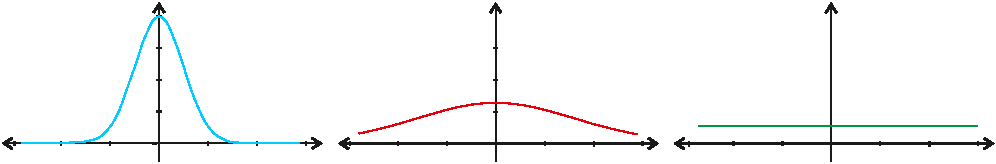
\includegraphics[width=10cm]{pictures/picture_2_4.pdf}};
    \draw [color=black](0,-4.7) node[anchor=north west] {$ c $};
    \draw [color=black](0,-1.6) node[anchor=north west] {$ \mu_{0} $};
    \draw [color=black](0,2.7) node[anchor=north west] {$ \mu_{0} $};
    \draw [color=black](3,4) node[anchor=north west] {$ \sigma^{2} = 1 $};
    \draw [color=black](3,0) node[anchor=north west] {$ \sigma^{2} = 10 $};
    \draw [color=black](3,-4) node[anchor=north west] {$ \sigma^{2} \rightarrow \infty $};
    \end{tikzpicture}
\end{center}
	
	Zkoumáme tedy hypotézu $\hypothesis{\t\in\Theta_0}{\t\notin\Theta_0}$. Máme k~dispozici $\X....T(\X)$, kde $T(\X)\sim\FF_T$. Testujeme tedy $W_\alpha=\big\{ |T(\X)|<K_\alpha \big\}$. Bayesova věta nám říká, že pokud je $\t$ znáhodněný parametr, potom pravděpodobnost, že platí $H_0$ je rovna ????? (tohle jsem nějak nestihnul).
	\end{enumerate}
\end{example}
\chapter{Princip postačitelnosti, podmíněnosti, věrohodnosti, zastavovací pravidlo sekvenčního principu, vztahy.}


\chapter{Bayesovský princip, bayesovský úplný model, výhody jeho použití, vztah k~ostatním principům.}


\chapter{Třídy optimálních strategii, užitková funkce a~podmínky pro~existenci užitkové funkce.}


\chapter{Bayesovské riziko, aposteriorní hustota, prediktivní bayesovská hustota.}


\chapter{Asymptotické vlastnosti aposteriorní hustoty a~bayesovských bodových odhadů.}


\chapter{Formy apriorní informace, princip neurčitosti, Jeffreysova hustota, ukázky.}


\chapter{Konjugované systémy apriorních hustot, princip maximální entropie, limitní aposteriorní hustoty, příklady.}


\chapter{Nejméně příznivá apriorní rozdělení, souvislost s~minimaxním principem rozhodování.}


\chapter{Přípustnost bayesovského řešení, Steinův efekt pro~sféricky symetrická rozdělení, Bergerův jev.}


\chapter{Grupy transformací, ekvivariantní odhady a~jejich bayesovská representace.}


\chapter{Bayesovské odhady pro~absolutní, multi-lineární, (váženou) kvadratickou a~0-1 ztrátovou funkci.}


\chapter{Hierarchický bayesovský model, empirický Bayes a~jeho suboptimalita, aplikace.}


\chapter{Laplaceova asymptotická expanze, podmínky regularity stochastické aproximace, numerické kvadratury.}


\chapter{Vzorkování podle důležitosti, Metropolisův algoritmus, variační Bayes.}


\chapter{Bayesovská strategie testování hypotéz, Bayes faktor, vlastnosti, porovnání s~klasickými testy.}



\chapter{Princip postačitelnosti, podmíněnosti, věrohodnosti, zastavovací pravidlo sekvenčního principu, vztahy.}
\begin{description}
	\item[SUFFICIENCY princip:] Máme $\epsilon$ závislé na~$\t$, pozorování $x,y$ a~nechť je v~$\epsilon$ k~dispozici postačující statistika $T$ (PS). Víme, že $T(x)=T(y)$ a~chceme, aby závěry o~$\t$ na~základě $x$ nebo $y$ byly shodné. ($T$ je PS pokud rozdělení $X|T(X)=t$ nezávisí na~$\t$).
	
	\item[LIKELIHOOD princip:] Informace o~$\t$ nesená $x$ je zcela obsažena ve~všech funkcích ($f_\X(\textbf{x},\t)=L$). Navíc, pokud máme pozorování $x_1$ experimentu $\epsilon_1$ a~$x_2$ v~experimentu $\epsilon_2$ taková, že 
	$$ L_1(\t|x_1)=c L_2(\t|x_2),\qquad\forall\t\in\Theta.$$
	Chceme, aby závěry o~parametru $\t$ v~obou experimentech byly shodné. označíme $\mathrm{Ev}(\epsilon_1,x_1)=\mathrm{Ev}(\epsilon_2,x_2)$ (Ev jako Evidence). 
	\item[CONDITIONALITY princip:] Nechť máme dostupné $\epsilon_1,\epsilon_2$. Definujeme $\epsilon^*$ experiment tak, že vybereme náhodně mezi~$\epsilon_1 \vee \epsilon_2$, a~v~něm měříme $x_1/x_2$. Chceme, aby $\Ev(\epsilon^*,(j,x_j))=\Ev(\epsilon_j,x_j),~\forall j,\forall x_j$.
	\item[STOPPING rule:] Máme $\epsilon_1,\epsilon_2$ jako zastavovací pravidlo $\tau$, které zastavuje posloupnost v~$\epsilon_n$. Jsou naměřeny $\textbf{x}=\Big( x_1^{\epsilon_1},x_2^{\epsilon_2},...,x_n^{\epsilon_n} \Big)$, ozn. $\{ \epsilon_1,...,\epsilon_n,\tau \}$ (sekvenční). Chceme, aby $\Ev\Big( \{ \epsilon_1,...,\epsilon_n,\tau \},\textbf{x} \Big)$ zvisela na~$\tau$ pouze prostřednictvím $\textbf{x}$, tzn. $$\Ev\Big( \{ \epsilon_1,...,\epsilon_n,\tau_1 \},\textbf{x} \Big)=\Ev\Big( \{ \epsilon_1,...,\epsilon_n,\tau_2 \},\textbf{x} \Big),~\forall \textbf{x}.$$
	\item[BAYESOVSKÝ princip:] Taková procedůra, která využívá k~rozhodnutí o~parametru $\t$ aposteriorní hustotu $\pi(\t,\textbf{x})=\frac{f_\X\cdot\pi(\t)}{\int f_\X\cdot\pi(\t) d\t}$, např. $\widehat{\t}_B=''\EE{\pi(\t,\textbf{x})}''=\E^\pi(\t)$.
\end{description}

\begin{example}[STOPPING rule]
	Mějme $\epsilon_j..x_j\in\Ran(X_j)$, kde $X_j\sim f(x_j,\t),~\forall j\in 1,2,...$. Teoricky můžeme jít až do~nekonečna, ale někdy chceme experiment zastavit, abychom mohli vyhodnotit data. Definujeme tedy $\tau$ jako zastavení v~bodě $n$, pokud $\textbf{x}:=(x_1,...,x_n)\in\Ran(X_1)\times\Ran(X_2)\times...\times\Ran(X_n)\equal{ozn}\Aa_n$. Platí, že
	$$ L(\t|\textbf{x})\equal{id}\Big(\prod f_{X_j}(x_j,\t) \Big)\cdot I_{\Aa_n}(\textbf{x})=f(x_1|\t)f(x_2|x_1,\t)...f(x_n|x_1,x_2,...,x_{n-1},\t)I_{\Aa_n}(\textbf{x}).$$
	dvě různá zastavovací pravidal $\tau_1,\tau_2$, která zastaví na~základě stejného $\textbf{x}(\epsilon_n)$ ve~stejném bodě (!! prosím o~intro). Pokud platí $L$ princip, potom platí $SR$ princip, tedy ($L_1^{(\tau_1)}=L_2^{(\tau_2)}$).
\end{example}
\begin{example}[BAYESOVSKÝ princip]
	Máme TV seriál. Označme $\t\in[0,1]$ jako podíl diváků, kteří daný seriál sledují. Bylo zjištěno, že 9 diváků seriál sledují a~3 nikoliv (to jsou naše data). Problém je, že nevíme, jakým způsobem byla data naměřena. 
	\begin{description}
		\item[$\epsilon_\mathrm{I}:$] vybráno $n=12$ lidí - test (9DIV,3NEDIV). Máme tedy náhodnou veličinu $X$ jako počet diváků z~$n=12$ nezávislých opakování. Z~toho plyne, že $X\sim \Bi(12,\t)$. Máme napozorováno $X(\omega)=x=9$.
		\item[$\epsilon_\mathrm{II}:$] vybíráme $N$ osob a~testujeme, dokud nezískáme $3$ nediváky. Při~tomto způsobu ale měření probíhá zcela odlišně. Tedy $N\sim\mathrm{NegBi}(3,1-\t)$. Napozorováno tedy bylo $N(\omega)=n=12$.
	\end{description}
	$$ L_\mathrm{I}(\t,\epsilon_\mathrm{I})=c_1\t^9(1-\t)^3\quad\propto\quad L_\mathrm{II}(\t,\epsilon_\mathrm{II})=c_2\t^9(1-\t)^3,\quad \forall\t\in[0,1] $$
	Z toho pro~LIKELIHOOD vyplývá, že $\Ev(\epsilon_\mathrm{I},(9))=\Ev(\epsilon_\mathrm{II},(12))$ (takže vlastně na~zastavovacím principu nezáleželo).
\end{example}

\begin{example}
	Máme laboratoř a~v~ní dva přístroje. Jako $\t$ označme\begin{itemize}
		\item 1. přístroj přesný $X_1\sim\NN(\t,0.1)$ [$\epsilon_1$] (vytížený)
		\item 2. přístroj nepřesný $X_2\sim\NN(\t,10)$ [$\epsilon_2$] (volný)
	\end{itemize}
	Rozhodování o~$\t$: 95\%-interval spolehlivosti pro~$\t$\begin{enumerate}[A)]
		\item osobně. naměříme $x_1$ jako délka($IS_{95\%}$)$=0.62$ (na 2.př. nezáviselo).
		\item vyšleme laborantku. která nese data (ale neví, ze~kterého přístroje jsou, prostě mohla použít i~volný přístroj). $\beta\in(0,1)$. Máme model $\Phi=\beta\NN(\t,0.1)+(1-\beta)\NN(\t,10).$ Pak zjistíme $x$ jako délku($IS_{95\%}$) s~hodnotou $5.19$.
	\end{enumerate}
\end{example}
\begin{theorem}
	$S\wedge C\Leftrightarrow L\Rightarrow SR$. Implikace $S\Rightarrow C$ je důležitá, protože $B~''\Rightarrow'' L$.
	\begin{proof}
		Mějme $\epsilon_1,\epsilon_2$, $x_1,x_2$ a~předpokládejme, že $L_1(\t)=c L_2(\t)$. Ptáme se, jestli je $\Ev(\epsilon_1,x_1)=\Ev(\epsilon_2,x_2)$. Víme, že $$ \underbrace{\pi_1(\t,x_1)}_{\epsilon_1}=\frac{f_X(x_1,\t)\pi(\t)}{\int f_X(x_1,\t)\pi(\t)\d\t}=\frac{c f_{X_2}\pi}{\int c f_{X_2}\pi\d\t}=\underbrace{\pi_2(\t| x_2)}_{\epsilon_2}.$$
	\end{proof}
	\begin{proof}[$L\Rightarrow S$]
		Nechť T je PS($\epsilon$) a~nechť máme data $x_1^0,x_2^0$ (nula značí konkrétní výběr, nikoliv obecný), taková, že $T(x_1^0)=T(x_2^0)$. Máme k~dispozici Neymannův faktorizační teorém, $X\sim f(x,\t)$, pak $T(X)$ je PS právě tehdy, když $f(x|\t)=h(x)g\big(T(x),\t \big),~\forall\t$. Potom tedy 
		$$ L(\t|x_1^0)=f(x_1^0,\t)=h(x_1^0)g\big( T(x_1^0),\t \big)=\frac{h(x_1^0)}{h(x_2^0)}\underbrace{h(x_2^0)g\big(T(x_2^0),\t \big)}_{f(x_2^0,\t)=L(\t,x_2^0)},\quad\forall\t.$$
		Z toho vyplývá (dle L principu), že $\Ev(\epsilon,x_1^0)=\Ev(\epsilon,x_2^0)$.
		
	\end{proof}
	\begin{proof}[$L\Rightarrow C$]
		Uvažujeme experiment $\epsilon^*$ tak, že $(\mathrm{I},X_\mathrm{I})=X^*$, $(\forall j\in\{1,2\},~\forall x_1,x_2)$, tedy $$\Ev\big(\epsilon^*,(j,x_j) \big)=\Ev\big(\epsilon_j,x_j \big).$$
		Dále potom $$ L^*(\t|\underbrace{j,x_j}_{X^*})=\PP\big(X^*=(j,x_j) \big)=\PP(I=j\wedge X_{I=j}=x_j)=\PP(I=j)\PP(X_j=x_j)=0.5f(x_j,\t)=0.5 L_j(\t,x_j).$$
		Potom 
		$$L^*=c L_j,~ \forall j,\forall x_j\quad\Rightarrow\quad\Ev\big(\epsilon^*,(j,x_j) \big)=\Ev\big(\epsilon_j,x_j \big).$$
	\end{proof}
\end{theorem}

Statistical decision theory:

\begin{define}
	Označíme $\Dd$ jako množinu možných rozhodnutí o~$\t$, případně $\tau(\t)$. Dále potom $\delta\in\Dd$. $L:\Theta\times\Dd\to[0,+\infty)$ nazýváme \textbf{loss function} (ztrátová funkce) a~$L(\t,\delta)$ jako \textbf{míru ztráty} (shody, neshody), pokud pro~$\t$ použijeme rozhodnutí $\delta$.
	
	Označme dále $\Rr$ jako \textbf{reward space}, který je spojen s~$\Dd$,tj. $\forall\delta\in\Dd$ přiřazuje $r\in\Rr$ ($\delta\leftrightarrow r$). Předpokládejme dále, že na~$\Rr$ existuje úplné uspořádání ($\leq$) tak, že \begin{enumerate}[A1)]
		\item $\forall r_1,r_2\in\Rr,~r_1\leq r_2 \vee r_2\leq r_1$,
		\item $\forall r_1,r_2,r_3\in\Rr,~r_1\leq r_2 \wedge r_2\leq r_3~\Rightarrow~r_1\leq r_3$. Z~toho vyplývá, že 
		$$ r_1<r_2,\quad r_2<r_1,\quad r_1=r_2~(r_1\sim r_2).$$
		Poslední rovnost není myšlena jako číselná rovnost, ale spíše jako ekvivalence (peníze pro~nás můžou mít stejnou cenu, jako získané znalosti).
	\end{enumerate}
	Nad $\Rr$ definujeme prostor $\mathcal{P}$ jako pravděpodobnostní distribuci $\{\PP\}$ nad~$r$ ($r\sim\PP\in\mathcal{P}$). Předpokládejme, že na~$\mathcal{P}$ existuje úplné uspořádání ($\leq$) takové, že ...
\end{define}

Motivace: označme $d_i$ jako investice do~$i$-té společnosti. Na~konci roku pak očekáváme dividenda $r_i$. $(d_i)_1^k...(r_i)_1^k...r_i\sim \PP_1\ast\PP_k$ (CLT)..

\section{15.10.}
\begin{define}
	Funkci $U$ na~$\R$ nazveme \textbf{užitkovou} (utility function), pokud $\forall P,Q\in\mathcal{P}$ platí, že 
	$$ P\leq Q\quad\Leftrightarrow\quad\E^P\big[U(r)\big]\leq\E^Q\big[U(r)\big],$$ kde $r$ je náhodná veličina. Pokut to jde, můžeme například definovat $U(r)=r$.
\end{define}
\begin{remark}
	Pokud má $\mathcal{P}$ vhodné vlastnosti, pak existuje užitková funkce $U(r)$, která zachovává dané uspořádání $\mathcal{P}$. 
\end{remark}
\begin{remark}
	\begin{enumerate}[a)]
		\item Pro~ztrátu $L(\t,\delta)$ platí, že $L(\t,\delta)=U(\t,\delta)=-\E[U(r)]+c$, kde konstantu $c$ přičítáme proto, abychom se~nedostali do~záporných čísel. Tím zajistíme, že pokud budeme provádět minimalizaci $L$, pak provádíme i~maximalizaci užitku.
		\item Předpověď počasí v~Kanadě. Předpovědi jsou ve~tvaru "pravděpodobnost, že zítra bude pršet je $p$". Předpovědi od~$N$ různých společností chceme nějak porovnat. Sledujeme tedy 365 dní všechny předpovědi a~přiřadíme jim $p_1,...,p_N$. Definujeme relativní četnost $$\t_j=\frac{\text{\# dnů, kdy pršelo a~byla použita }p_j}{\text{\# dnů, kdy byla použita }p_j},j\in\widehat{N}.$$ Sestavíme ztrátovou funkci (poprvé použil De Grout v~roce 1988) $$L(\t,p)=\sumjn q_j(\underbrace{p_j-\t_j}_{H(q)})^2+\sum_{i=1}^N q_i\ln q_i,$$ kde $q_j=\frac{\text{\# použití }p_j}{365}$ a~$H(q)=-\sum_1^J q_j\ln q_j\geq 0$, kde ${q_j}_1^J$ jsou rozdělení pravděpodobnosti. Suma $\sum_{i=1}^N q_i\ln q_i$ pak penalizuje předpovědi, které jsou nevyvážené.
		
		Pokud bychom měli systém neuspořádanosti, pak by bylo $H(\textbf{q})$ maximální. O~$\textbf{q}$ víme, e má rovnoměrné rozdělení $q_j=\frac{1}{J}$.
	\end{enumerate}
\end{remark}
\begin{remark}
	Člen $\sumjn q_j(p_j-\t_j)^2$ v~minulé poznámce nemusí nutně být na~druhou, můžeme brát závorku i~v~absolutní hodnotě, případně ji umocnit na~$\alpha$. Zde vstupuju do~našeho problému tzv. \textbf{Apriorno}. Musíme totiž dopředu vědět některé informace, třeba $X\sim f(x,\t),~L(\t,\delta)$.
\end{remark}
\begin{define}
	Mějme $\Theta$, $\mathcal{F}=\big\{ f(x,\t):\t\in\Theta \big\}$,~$\mathscr{D}$, kde $\delta\in\mathscr{D}$ a~$\chi$ jako výběrový prostor s~daty $\textbf{x}$.
	
	Funkci $\delta:\chi\to\mathscr{D}$ nazýváme \textbf{rozhodovací funkce}, $\delta(\textbf{x})=\delta\in\mathscr{D}$. 
\end{define}
\begin{description}
	\item[Metoda A) minimalizace L] Máme $\delta_L(\textbf{x})=\argmin\limits_{\delta\in\mathscr{D}} L\big(\t,\delta(\textbf{x})\big),~\forall \t\in\Theta,~\forall\textbf{x}\in\chi$. (vynechal jsem prezentace)
	\item[Metoda B) Riziková funkce] (risk function) je funkce $\mathcal{R}:\Theta\to\R^+$ definovaná jako $$\mathcal{R}(\t,\delta)=\E_\t L\big(\t,\delta(\textbf{X})\big)=\int L\big(\t,\delta(\textbf{x})\big)f_\textbf{X}(\textbf{x},\t)\d\textbf{x}.$$
	Rizikovou funkci také nazýváme jako \textit{střední ztrátu}. Dále definujeme $\delta_U=\argmin\limits_{\delta\in\mathscr{D}} \mathcal{R}(\t,\delta),~\forall\t\in\Theta$.
	\begin{figure}[h]
	\centering
    \begin{tikzpicture}
    \node[inner sep=0pt] (pic) at (0,0)
    {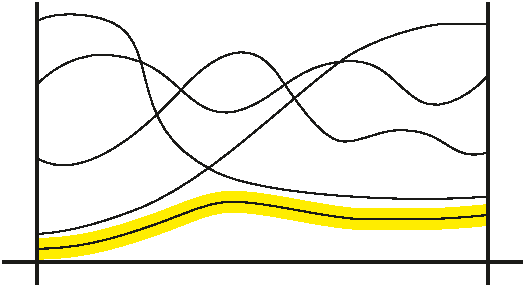
\includegraphics[width=7.5cm]{pictures/picture_3_2.pdf}};
    \draw [color=black](3.4,2.2) node[anchor=north west] {$ \text{R}(\theta, \delta_1 )
     $};
     \draw [color=black](3.4,1.2) node[anchor=north west] {$ \text{R}(\theta, \delta_2 )
     $};
    \end{tikzpicture}
    \caption{HPD Region.}
\end{figure}
	
	Ne vždy lze najít stejnoměrně nejlepší řešení. V~takovém případě pak přejdeme na~prostor $\mathscr{D}_0\subset\mathscr{D}$, kde již lze najít stejnoměrně nejlepší řešení (typicky vypustíme některé rizikové funkce). Můžeme tedy brát různé prostory rozhodovacích fukncí:
	\begin{enumerate}[a)]
		\item  Prostor rozhodovacích funkcí, které jsou nestranné -- pak vede na~UMVUE.
		\item $\mathscr{D}_0$ takový, který je prostorem rozhodovacích funkcí invariantních na~určitou transformaci (např. posunutí, přeškálování -- lokálně-měřítkové modely).
	\end{enumerate}
	
	Problémy: \begin{enumerate}[a)]
		\item $\delta_1,\delta_2$ a~k~nim $\mathcal{R}(\t,\delta_1),\mathcal{R}(\t,\delta_2)$ takové, že se~kříží -- nejsme schopni rozhodnout, která strategie je lepší.
		\item Minimalizujeme $\E L$, ale předpis $\delta$ (odhadce) nezávisí na~$\textbf{x}$ - výběr nejlepšího $\delta$ nezávisí na~naměřených datech.
		\item Na~rozmyšlenou je následující příklad \ref{example:problemy}.
	\end{enumerate}
\end{description}

\begin{example} \label{example:problemy}
	Mějme $X=\begin{cases}
	\t-1,& \PP=\frac{1}{2}, \\ \t+1,& \PP=\frac{1}{2},
	\end{cases}~\t\in\R,~\mathscr{D}=\R$. Potom
	$ L(\t,\delta)=1-I_\t(\delta)$ nazýváme "0-1" ztrátovou funkci, viz obrázek \ref{pic11}.
	
	\begin{figure}[h]
	\centering
    \begin{tikzpicture}
    \node[inner sep=0pt] (pic) at (0,0)
    {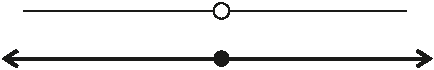
\includegraphics[width=7.5cm]{pictures/picture_3_3.pdf}};
    \draw [color=black](3,0.4) node[anchor=north west] {$ \delta $};
     \draw [color=black](0,-0.5) node[anchor=north west] {$ \theta $};
    \end{tikzpicture}
    \caption{Doplnit popisek :)}
\end{figure}	
	
	\begin{enumerate}[1)]
		\item Máme $(x_1,x_2)$ data a~sestrojíme $\delta_0=\frac{x_1+x_2}{2}=\begin{cases}
		\t\\\t-1\\\t+1
		\end{cases}$ symetricky kolem~$\t$. Potom
		$$ \mathcal{R}(\t,\delta_0)=\E L(\t,\delta_0)=1-\E I_\t(\delta_0)=1-\PP(\delta_0=\t)=1-\PP(X_1\neq X_2)=\frac{1}{2}.$$ To nám říká, že střední ztráta je rovna $\frac{1}{2}$. V~průměru tedy 50\% případu bude příznivá (trefíme se~do~parametru).
		\item Máme data $(x_1,x_2)$ a~sestrojíme $\delta_1=x_1+1=\begin{cases}
		\t\\\t+2
		\end{cases}$ nesymetricky rozdělené kolem~$\t$. Potom
		$$\mathcal{R}(\t,\delta_1)=...=1-\PP(\delta_1=\t).$$
	\end{enumerate}
	Srovnání $\delta_0$ a~$\delta_1$ nelze rozhodnout na~základě $\mathcal{R}$-strategie. Můžeme na~ně však využít např. UMVUE, MREE nebo N-P lemma.
\end{example}
\begin{description}
	\item[Metoda c) Strategie MINIMAXní] $\sup\limits_{\t\in\Theta} \mathcal{R}(\t,\delta)$ nazýváme ''\textit{maxní}''(\textit{supremální}) riziková funkce a~je rovna $\mathcal{R}_{\sup}(\t,\delta)$. Definujeme 
	$$ \delta_0=\argmin\limits_{\delta\in\mathscr{D}}\mathcal{R}_{\sup}(\t,\delta)=\argmin\limits_{\delta\in\mathscr{D}}\underbrace{\sup\limits_{\t\in\Theta}\underbrace{\E_\t L(\t,\delta(\X))}_{\mathcal{R}(\t,\delta)}}_{r_{\sup}\in\R_0^+}.$$
\end{description}

\begin{define}
	Definujeme \textbf{minimaxní riziko} ve~tvaru $\overline{\mathcal{R}}=\inf\limits_\delta\sup\limits_\t\mathcal{R}(\t,\delta)$.
\end{define}

\begin{figure}[h]
	\centering
    \begin{tikzpicture}
    \node[inner sep=0pt] (pic) at (0,0)
    {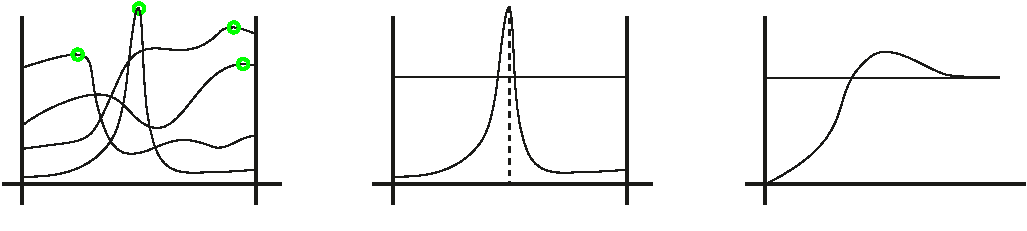
\includegraphics[width=15.0cm]{pictures/picture_3_4.pdf}};
    \draw [color=black](3,0.5) node[anchor=north west] {$ \delta $};
     \draw [color=black](0,-0.3) node[anchor=north west] {$ \theta $};
    \end{tikzpicture}
    \caption{1: zeleně suprema, nejmenší supremum je delta3 2: lepší je delta2, protože ač je riziko vysoké, jeho šance je velice malá - toto je nevýhoda minimaxní strategie 3: delta2 jen lehce překmitne delta1 a~pak se~k~němu blíží asymptoticky}
\end{figure}





\begin{remark}
	Analogie z~teorie her. Pokud máme 2 hráče, kteří mají antagonický vztah (snaží se~navzájem poškodit a~nezáleží jim na~ztrátě). První hráč udělá nějaký tah. Druhý hráč pak udělá tah, který co nejvíc poškodí 1. hráče. První hráč to předvídá a~snaží se~tedy minimalizovat nejhorší možnou ztrátu.
\end{remark}

\begin{remark}
	Stavba naftové plošina v~Severním moři. Máme vstupy=parametry (teplota, vítr, příliv, bouřky, lidský faktor,...) a~rozhodujeme se, jak plošinu postavit.
	\begin{figure}[h]
		\centering
		\begin{tikzpicture}[line cap=round,line join=round,>=triangle 45,x=1.5cm,y=1.5cm]
		\clip(-1.25,-0.27) rectangle (7,3.03);
		\draw [->] (0,-0.48) -- (0,3);
		\draw [->] (-0.25,0) -- (5,0);
		\draw [dash pattern=on 2pt off 2pt] (4.27,-0.38)-- (4.27,2.55);
		\draw [dash pattern=on 2pt off 2pt] (-0.25,2.55)-- (4.27,2.55);
		\draw [shift={(0.04,2.55)}] plot[domain=-1.595:0,variable=\t]({1*0.63*cos(\t r)+0*0.63*sin(\t r)},{0*0.63*cos(\t r)+1*0.63*sin(\t r)});
		\draw [shift={(0.02,0)}] plot[domain=0:1.595,variable=\t]({1*0.74*cos(\t r)+0*0.74*sin(\t r)},{0*0.74*cos(\t r)+1*0.74*sin(\t r)});
		\begin{scriptsize}
		\draw [color=black] (1.64,1.4)-- ++(-1.5pt,-1.5pt) -- ++(3.0pt,3.0pt) ++(-3.0pt,0) -- ++(3.0pt,-3.0pt);
		\draw [color=black] (0.88,1.52)-- ++(-1.5pt,-1.5pt) -- ++(3.0pt,3.0pt) ++(-3.0pt,0) -- ++(3.0pt,-3.0pt);
		\draw [color=black] (1.98,1.9)-- ++(-1.5pt,-1.5pt) -- ++(3.0pt,3.0pt) ++(-3.0pt,0) -- ++(3.0pt,-3.0pt);
		\draw [color=black] (0.4,0.34)-- ++(-1.5pt,-1.5pt) -- ++(3.0pt,3.0pt) ++(-3.0pt,0) -- ++(3.0pt,-3.0pt);
		\draw [color=black] (3.2,1.8)-- ++(-1.5pt,-1.5pt) -- ++(3.0pt,3.0pt) ++(-3.0pt,0) -- ++(3.0pt,-3.0pt);
		\draw [color=black] (3.14,0.96)-- ++(-1.5pt,-1.5pt) -- ++(3.0pt,3.0pt) ++(-3.0pt,0) -- ++(3.0pt,-3.0pt);
		\draw [color=black] (1.98,0.52)-- ++(-1.5pt,-1.5pt) -- ++(3.0pt,3.0pt) ++(-3.0pt,0) -- ++(3.0pt,-3.0pt);
		\draw [color=black] (0.98,1.96)-- ++(-1.5pt,-1.5pt) -- ++(3.0pt,3.0pt) ++(-3.0pt,0) -- ++(3.0pt,-3.0pt);
		\end{scriptsize}
		\draw [color=black](-0.6,2.3) node[anchor=north west] {$ v_{\text{max}}$};
		\draw [color=black](-0.6,3) node[anchor=north west] {vítr};
		\draw [color=black](0,0) node[anchor=north west] {$ t_\text{min} $};
		\draw [color=black](3.3,0) node[anchor=north west] {$ +50^\circ C $};
		\draw [color=black](5,0.2) node[anchor=north west] {teplota};
		\draw [color=black](-0.4,0.4) node[anchor=north west] {$ 0 $};
		\end{tikzpicture}
		\caption{}
		\label{fig:p51}
	\end{figure}
	
\end{remark}
\begin{description}
	\item[Metoda d) Bayesovská riziková funkce] $r(\pi,\delta):\Pi=\{ \pi\text{ apriorní rozdělení pro~}\t \}\times\mathscr{D}\to\R_0^+$.
	$$ r(\pi,\delta)=\E^\pi\big[ R(\t,\delta) \big]=\int\limits_{\Theta}R(\t,\delta)\pi(\t)\d\t=\int\limits_{\Theta}\Big( \int\limits_{\chi}L\big(\t,\delta(\textbf{X})\big)f_\textbf{X}\d\textbf{x} \Big)\pi(\t)\d\t.$$
	Definujeme $\delta^\pi=\argmin\limits_{\delta\in\mathscr{D}}r(\pi,\delta)$, za~předpokladu existence, jako \textbf{Bayesovskou rozhodovací funkci}. Číslo $r(\pi)=r(\pi,\delta^\pi)$ nazýváme \textbf{Bayesovské (apriorní) riziko}.  
\end{description}
\begin{remark}
	Mějme $\pi$ fixní, $\delta_1\leq\delta_2~\Leftrightarrow~r(\pi,\delta_1)\leq r(\pi,\delta_2)$ uspořádané v~$\R^1$. Rozšíření i~na~\textbf{nevlastní apriorní hustoty} (inf.), pokud $r(\pi)<+\infty$. ($r_\text{inf}(\pi)=\inf_\delta r(\pi,\delta)<+\infty$)
\end{remark}
\begin{example}
	Mějme $X\sim\underbrace{\NN(\t,1)}_{f_X}$, $\t\in\R,~\pi(\t)=1$ (konstantní) na~$\R$ (nevlastní hustota). Pak
	$$ \pi(\t,|x)=\frac{f_X \pi(\t)}{\int_{-\infty}^{+\infty}f_X \pi(\t)\d\t}=\frac{1}{c}\e{-\frac{1}{2}(\t-x)^2}=\frac{1}{\sqrt{2\pi}}\e{-\frac{1}{2}(\t-x)^2}.$$
	\[\begin{split}
	\delta^\pi(\textbf{x})&=\EE{\pi(\t|x)}=\E\NN(x,1)=x\text{ obecněji }\overline{x}_n\\
	r(\pi)&= r(\pi,\delta^\pi)=\E^\pi R=\E^\pi[\E^f L_2]\equal{def}\E^\pi\big[ \E^f\underbrace{\big(\t-\delta^\pi(X) \big)^2}_{L_2} \big]=\E^\pi\E^f(\t-X)^2=\\&=\E^\pi\big[ \E^f(X-\E^fX)^2 \big]=\E^\pi(\sigma^2)=\int_{-\infty}^{+\infty}\sigma^2\cdot 1\d\t=+\infty
	\end{split}
	\]
\end{example}
\begin{define}
	Máme $L,~f_X,~\pi(\t)$. Definujeme \textbf{aposteriorní Bayesovskou rizikovou funkci} vztahem
	$$ \rho(\pi,\delta|\textbf{x})=\E^\pi\big[ L\big(\t,\delta(\textbf{x})\big)|\textbf{x} \big]=\int L\big(\t,\delta(\textbf{x})\big)\pi(\t|\textbf{x})\d\t.$$ 
\end{define}

\begin{description}
	\item[Metoda e) ???] definujeme $\delta_\rho^\pi(\textbf{x})=\argmin\limits_{\delta(\textbf{x})}\rho(\pi,\delta(\textbf{x})|\textbf{x})$ za~předpokladu existence pro~skoro všechna $\textbf{x}$.
\end{description}

\begin{remark}
	Výhoda tého definice je, že $\delta_\rho^\pi$ závisí přímo na~datech $\textbf{x}$. Nevýhoda pak je, že musíme minimalizaci dělat opakovaně pro~každá data $\textbf{x}$.
\end{remark}
\begin{theorem}
	Mám-li $\delta_\rho^\pi~\forall s.v.\textbf{x}$, pak $/delta_\rho^\pi=\delta^\pi$ Bayesovskou rizikovou funkci (D strategie $\delta^\pi=\argmin_\delta r(\pi,\delta)$).
	\begin{proof}
		\[
		\begin{split}
		\rho\big(\pi,\delta_\rho^\pi(\textbf{x})|\textbf{x}\big)&\leq \rho(\pi,\delta(\textbf{x})|\textbf{x}), \\
		\E^m\rho\big(\pi,\delta_\rho^\pi(\textbf{x})|\textbf{x}\big)&\leq \E^m\rho(\pi,\delta(\textbf{x})|\textbf{x}),
		\end{split}
		\]
		kde
		\[
		\begin{split}
		\E^m\rho(\pi,\delta(\textbf{x})|\textbf{x})&=\int\limits_{\chi}\Big( \int\limits_{\Theta} L(\t,\delta)\underbrace{\pi(\t|\textbf{x})}_{\frac{f\pi(\t)}{\int f\pi(\t)\d\t}=\frac{f\pi(\t)}{m(\textbf{x})}}m(\textbf{x})\d\textbf{x}\Big)\equal{Fubini}\int\limits_{\Theta}\Big( \underbrace{\int\limits_{\chi} L\big(\t,\delta(\textbf{x})\big)f(\textbf{x}|\t)\d\textbf{x}}_{\E^f L=R(\t,\delta)} \Big)\pi(\t)\d\t=\\&=\E^\pi\E^f L=r(\pi,\delta) 
		\end{split}
		\]
		a tedy 
		$$ r(\pi,\delta_\rho^\pi)\leq r(\pi,\delta),~\forall\delta\quad \Rightarrow\quad \delta_\rho^\pi=\delta^\pi.$$
		Závěr: D strategie Bayes($\delta^\pi$) je rovna E strategii Bayes ($\delta_\rho^\pi(\textbf{x})$ skoro všude $\textbf{x}$).
	\end{proof} 
\end{theorem}
Rozšíření: máme $\delta_\rho^\pi(\textbf{x}),~\forall s.v.~ \textbf{x}$ a~stane se, že $r(\pi)=+\infty$. Toto řešení nazveme \textbf{Zobecněnou Bayesovskou rozhodovací funkcí}.

Další výhody: $\pi(\t)$ a~máme data $\textbf{X}\sim f(\textbf{x},\t)\stackrel{\text{ÚBM}}{\longrightarrow}\pi(\t,\textbf{x})$ (ÚBM = úplný Bayes. model) update ($\widehat{\t}_B$ int. spol.). $\tilde{\pi}(\t)=\pi(\t|\textbf{x})$ nová data $\tilde{\textbf{X}}\sim\tilde{f}(\tilde{\textbf{x}}|\t)\stackrel{\text{ÚBM}}{\longrightarrow}\tilde{\pi}(\t|\tilde{\textbf{x}})$ update ($\tilde{\widehat{\t}_B}$) apod. 

\begin{example}
	Varianta: lékař sleduje chorobu pacienta. 1. den $x_1\sim f(x|\t)$, kde $\pi_1(\t)$ je apriorní informace. Z~toho pak $\pi(\t|x_1)$. 2. den naměří $x_2\sim f(x|\t)$. Z~toho pak $\pi_2(\t)=\alpha\pi(\t| x_1)+(1-\alpha)\tilde{\pi}_2(\t)\to \pi(\t|x_2,x_1)$. n-tý den pak neměří $x_n$ a~proces se~opakuje.
\end{example}
\subsection*{Úloha predikce}
\begin{description}
	\item[KLAS. STAT.] Máme $X\sim f(x,\t)$, data $D\sim\textbf{x}=(x_1,...,x_n)$, realizaci $\textbf{X}=(X_1,...,X_n)$ a~hledáme predikci $X_{n+1}$. Pokud použijeme IID model, pak $X_{n+1}\sim f(x|\t)$ a~odhad $\widehat{\t}=\widehat{\t}(\textbf{x})=\widehat{\t}_{\mathrm{ML}}$. Z~toho pak $\widehat{f}(x)=f(x,\widehat{\t}_\mathrm{ML})$ a~z~toho $X_{n+1}\sim\widehat{f}$.
	\item[BAYES. STAT.] \begin{enumerate}[a)]
		\item Máme $X\sim f(x|\t)$, data $D:\textbf{x}$ a~$\pi(\t)$ apriorní informaci. Z~toho získáme $\pi(\t|\textbf{x})$ a~z~toho $\widehat{\t}_B=\EE{\pi(\t|\textbf{x})}$. Z~toho už $\widehat{f}(x)=f(x|\widehat{\t}_B)$ a~potom $X_{n+1}\sim\widehat{f}$.
		\item $\tau(\t)=f(x|\t)$, $\pi(\t)$, $\widehat{f}_B(x)=\widehat{\tau(\t)_B}$... $X_{n+1}\sim\widehat{f}_B$.
		\item Definujeme ÚBM $X\sim f_X(x|\t)$, $\pi(\t)$, $\pi(\t|\textbf{x})$. Pak definujeme \textbf{Bayesovskou prediktivní hustotu} $f_B^{PR} $ vztahem
		$$ f_B^{PR}(t|\textbf{x}\sim\text{data})=\int\limits_{\Theta} \underbrace{f_X(t|\t)\pi(\t,\textbf{x})}_{\phi(t,\t|\textbf{x})}\d\t=\EE{f_X(t|\t)|\textbf{x}}.$$
		Potom
		$$ X_{n+1}\sim f_B^{PR}(x_{n+1}|\textbf{x}\text{ data})\quad\to\quad \PP(X_{n+1}>b)=\int\limits_b^{+\infty}f_B^{PR}\d x_{n+1}.$$
		Výhodou je potom to, že obsahuje plnou informaci ve~tvaru $\pi(\t|\textbf{x})$.
	\end{enumerate}
\end{description}
\begin{define}
	Mějme $P,Q\in\mathcal{P}$ a~definujeme \textbf{totální variaci} $\TV(P,Q)=\left\|P-Q\right\|_\TV=\sup\limits_{|g|\leq 1}\left| \int g(\X)\d P-\int g(\Y)\d Q \right|\equal{ASR}=\left|\begin{array}{l}
	p\equal{ozn}\frac{\d P}{\d \mu}\quad P,Q\ll\mu\\ q=\frac{\d Q}{\d \mu}
	\end{array}
	\right|=\int |p-q|\d\mu=\left\|p-q\right\|_{L_1}$.
\end{define}
\begin{define}
	Mějme $(P_n)_1^{+\infty},~Q$. Řekneme, že $P_n\stackrel{\text{silně}}{\longrightarrow}Q$, pokud $\TV(P_n,Q)\to0$.
\end{define}
\begin{remark}
	$$ P_n\wto Q~\Leftrightarrow~\int g(\X)\d P_n\to\int g(\Y)\d Q,\qquad \forall g\in C_B^{(0)}\text{ spojité a~omezené.}$$
\end{remark}
\begin{theorem}
	Nechť $P_n\stackrel{s}{\to}Q\Rightarrow P_n\wto Q$ (AN). Funkce $g$ nechť je spojitá a~omezená, $|g|\leq M$. $g^\ast =g|_M$, $|g^\ast|\leq 1$. Pak
	$$ \left| \int g(\X)\d P_n-\int g(\Y)\d Q \right|=M\left| \int g^\ast(\X)\d P_n-\int g^\ast(\Y)\d Q \right|\leq M\cdot \left\| P-Q\right\|_\TV\to0.$$
\end{theorem}
\begin{theorem}[Scheffé theorem]
	Mějme $P_n,Q$ s~ASR$_\mu$, $p_n=\frac{\d P_n}{\d \mu}$, $q=\frac{\d Q}{\d \mu}$. Nechť dále $p_n\to q~s.v.\mu$. Pak $P_n\stackrel{s,(\TV)}{\longrightarrow}Q$. 
	\begin{proof}
		$$ \left| \int_A (p_n-q)\d\mu \right|\leq \int_A|p_n-q|\d\mu\leq \int_\R|p_n-q|\d\mu=2\int(p_n-q)^+\d\mu\to0,$$
		kde poslední rovnost platí, protože $\int(p_n-q)\d\mu=0$, a~tedy $\int(p_n-q)^+\d\mu-\int(p_n-q)^-\d\mu=0$.	\end{proof}
\end{theorem}
\begin{remark}
	Opakování. Z~01MAS víme, že pro~$\fregmle$ platí, že \begin{enumerate}[1)]
		\item $\supp f$ nezávisí na~$\t$,
		\item $f\in\mathcal{C}^{(3)}$ vzhledem k~$\t$ pro~$s.v.x\in\supp f$,
		\item $\int f_\t'=0$ a~$\int f_{\t\t}''=0$,
		\item $\left( \mathbb{J}(\t)_{(\text{FIM})} \right)_{i,j}=\EE{\frac{\partial\log f}{\partial \t_i}\cdot\frac{\partial\log f}{\partial \t_j}}=-\EE{\frac{\partial^2 \log f}{\partial\t_i \partial \t_j}}$, $\mathbb{J}(\t)$ je PD a~konečná pro~$\forall\t\in\Theta$,
		\item $\forall\t_0~\exists H_{\t_0}~\exists M(\X)\in\LL_1(P_{\t_0})$ tak, že $\left\| \frac{\partial^3\log }{\partial \t^3}\right\|\leq M(x)$ na~$H_{\t_0}$, kde $\E_{\t_0}[M(X)]<+\infty$.
	\end{enumerate}
\end{remark}
\begin{theorem}[Bernstein - von Mises]
	Předpokládejme ÚBM: $X\sim f(x|\t)~w.r.t.\lambda,\sigma-$finite, $\mathcal{F}=\left\{ f(x|\t):\t\in\Theta\subset R^k \right\}$, $\Theta$ otevřená, $\t\sim\pi(\t)$ vlastní hustota spojitá (Tedy máme $\Phi(x,\t)=f\cdot\pi$, $m(\textbf{x})=\int f\cdot \pi\d\t$, $\pi(\t|\textbf{x})=\Phi/m=\frac{f\cdot\pi}{\int f\cdot\pi\d\t}$). Nechť dále $\mathcal{F}=\fregmle$. Pak
	$$ \left\| \pi_n(\t|\textbf{x})-f_{\NN\left( \widehat{\t}_n,\frac{1}{n}\mathbb{J}^{-1}(\t) \right)} \right\|\to0,$$
	kde $\widehat{\t}_n$ je konzistentní řešení $LE_Q$, tzn. $\widehat{\t}_n$ řeší $\frac{\partial \log f}{\partial \t_j}=0,~\forall j\in\hat{k}$.
\end{theorem}
\begin{dusl}
	Mějme $\fregmle$, $\pi(\t)>0$ spojitá, $\t_0$ skutečná hodnota parametru $\t$. Pak $(\t|\textbf{x})\sim\AN\big(\htn(\textbf{x}),\frac{1}{n}\mathbb{J}^{-1}(\t_0)\big)$ pro~$\forall\t_0$.
	
	Závěr: $\sqrt{n}\big( (\t|\textbf{x})-\htn(\textbf{x}) \big)\Dto \NN\big( 0,\frac{1}{n}\mathbb{J}^{-1}(\t_0) \big),~\forall\t_0$. Bayesová strategie je asymptoticky ekvivalentní MLE.
	\begin{proof}
		$k=1$: Máme $f_x,~(X_j)_1^n,~f_{X_j}(x_j|\t),~f_n\equal{id}\prod_1^n f_{X_j}=f_n(\textbf{x}|\t),~\pi(\textbf{x}|\t),~\pi(\t|\textbf{x})=\frac{f_n \pi}{\int f_n \pi\d\t}$. Víme, že $(\t|\textbf{x})\sim\pi(\t|\textbf{x})$. Transformujeme pomocí $g: t=\sqrt{n}\big( \t|_\textbf{x}-\htn \big)$, $g^{-1}:\t|\textbf{x}=\htn + \frac{t}{\sqrt{n}}$, $\mathbb{J}_{g^{-1}}=\frac{1}{\sqrt{n}}>0$. Potom
		\[
		\begin{split}
		T&=\sqrt{n}\big(\t|_\textbf{x}-\htn\big)\stackrel{ozn.}{\sim}\pi(t|\textbf{x})=\frac{f_n\big(\textbf{x}|\htn+\frac{t}{\sqrt{n}}\big)\pi\big( \htn+\frac{t}{\sqrt{n}} \big)\big(\frac{1}{\sqrt{n}}\big)}{\int f_n(\textbf{x}|\t)\pi(\t)\d\t}=\left|\begin{array}{l}
		\t=\htn+\frac{s}{\sqrt{n}}\\\d\t=\frac{\d s}{\sqrt{n}}\end{array}
		\right|=\\ &=\frac{f_n\big(\textbf{x}|\htn+\frac{t}{\sqrt{n}}\big)\pi\big( \htn+\frac{t}{\sqrt{n}} \big)}{\int f_n\big(\textbf{x}|\htn+\frac{s}{\sqrt{n}}\big)\pi\big( \htn+\frac{s}{\sqrt{n}} \big)\d s}.
		\end{split}
		\]
		máme spojité $\partial_\t^3$, a~proto rozvineme $\log f_n$ do~2. řádu:
		\[
		\begin{split}
		\log f_n(\textbf{x}|\htn+\frac{t}{\sqrt{n}})&=\log f_n(\textbf{x}|\htn)+0+\frac{1}{2}\frac{t^2}{n}\frac{\partial^2 \log f_n}{\partial\t^2}\Big|_{\t=\htn}+R_n=\\&=\log f_n(\textbf{x}|\htn)+\frac{t^2}{2}\underbrace{\Big( \frac{1}{n}\sumjn \frac{\partial^2 \log f_{X_j}(x_j|\htn)}{\partial\t^2} \Big)}_{\stackrel{\PP_{\t_0}}{\longrightarrow}\EE{\frac{\partial^2\log f_X}{\partial\t^2}}=-\mathbb{J}(\t_0)}+R_n\stackrel{\PP_{\t_0}~s.j.}{\longrightarrow}0.
		\end{split}
		\]
		Z toho potom plyne, že $f_n\big(\textbf{x}|\htn+\frac{t}{\sqrt{n}}\big)=f_n(\textbf{x}|\htn)\e{-\frac{t^2}{2}\mathbb{J}(\htn)}\cdot\tilde{R}_n$ a~tedy \[
		\begin{split}
		\pi(t|\textbf{x})&=\frac{f_n\e{-\frac{t^2}{2}\mathbb{J}(\htn)}\cdot\tilde{R}_n \pi\big( \htn+\frac{t}{\sqrt{n}} \big)}{f_n\int \e{-\frac{s^2}{2}\mathbb{J}(\htn)}\tilde{R}_n \pi\big(\htn+\frac{s}{\sqrt{n}}\big)\d s}\stackrel{\PP_{\t_0}}{\to}\frac{\e{-\frac{t^2}{2}\mathbb{J}(\t_0)}\cdot1\cdot \pi(\t_0)}{\int\e{-\frac{s^2}{2}\mathbb{J}(\t_0)}\cdot1\cdot\pi(\t_0)\d s}=\left| \begin{array}{l}
		u=s\sqrt{\mathbb{J}(\t_0)}\\\d s=\frac{\d u}{\sqrt{\mathbb{J}(\t_0)}}		
		\end{array}
		\right|=\\&=\frac{\sqrt{\mathbb{J}(\t_0)}}{\sqrt{2\pi}}\e{-\frac{t^2}{2}\mathbb{J}(\t_0)}\sim\NN\Big( 0,\frac{1}{\mathbb{J}(\t_0)} \Big).
		\end{split}
		\]
	\end{proof}
\end{dusl}
\begin{theorem}
	Mějme UBM, $f_X$, $\pi(\t)$ omezenou a~vlastní. Označme $\pi(\t|\textbf{x})=\frac{f\cdot\pi}{\int f\cdot\pi\d\t},~\pi_0(\t|\textbf{x})=\frac{f\cdot1}{\int f\cdot1 \d\t}$, kde $\int f\cdot\pi\d\t<+\infty$ a~$\int f\cdot1 \d\t<+\infty$. Pak
	$$ \left\|\pi(\t|\textbf{x})-\pi_0(\t|\textbf{x})\right\|_\TV\leq \max\Big(\frac{a+b}{1-a},\frac{a+b+ac}{1+a+b+ac}\Big)+\frac{a(2-a+c)}{1-a}=\epsilon_{a,b,c},$$
	kde $a,b,c$, $a\in[0,1),~b>0,~c>0$, jsou definovány následovně:\begin{enumerate}[1)]
		\item $\exists A\subset \Theta$ tak, že $\int_A \pi_0(\t|\textbf{x})\d\t\geq 1-a$,
		\item $\int_A \pi(\t)=m>0$,
		\item $\sup_A \pi(\t)\leq (1+b)m$,
		\item $\sup\limits_{\Theta\setminus A} \pi(\t)\leq(1+c)m$. 
	\end{enumerate}
\end{theorem}
\begin{dusl}
	Pokud dokážeme stlačit horní hranici $\epsilon_{a,b,c}$ k~nule, tak v~$\TV$ je $\pi(\t|\textbf{x})$ a~$\pi_0(\t|\textbf{x})$ velmi blízko. Potom tedy $\widehat{\t}_B^\pi=\EE{\pi(\t|\textbf{x})}$ a~$\widehat{\t}_B^1=\EE{\pi_0(\t|\textbf{x})}$. To znamená, že vliv $\pi(\t)$ se~ztrácí.
\end{dusl}\newpage
\begin{remark}
	$\epsilon_{a,b,c}$ chceme malé. Potřebujeme $a,b$ malé, $c$ ne příliš velké.
	
	\begin{figure}[h]
		\centering
		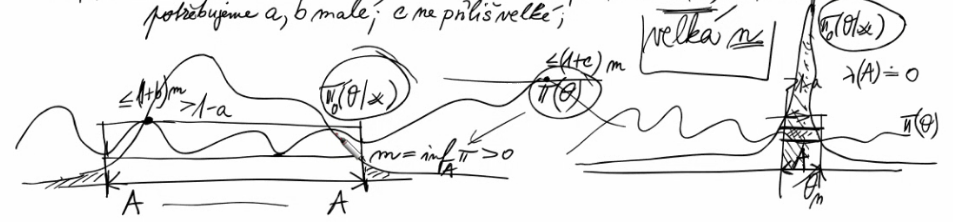
\includegraphics[width=0.95\linewidth]{pictures/P6_1}
		\caption{popis}
		\label{fig:p61}
	\end{figure}
	
\end{remark}

\section{5.11.}
Problém principu neurčitosti: $\pi(\t)=$konst. na~$\Theta$ (rovnoměrnou apriorní informaci).
\begin{example}
	Mějme $X\sim f(x|\t),~\t\in(0,1),~\pi(\t)=1$ na~$(0,1)$. Bayes: $\pi(\t|\textbf{x})$.. $\widehat{\t}_B(\textbf{x})$. Označme $\eta=\t^2...,~\t=\sqrt{\eta}$, reparametrizace $f(x|\t=\sqrt{\eta})=f(x|\eta)$. $\t$ považujeme za~znáhodněné (apriorně předpokládáme, že o~$\t$ nic nevíme). Transformace $\t$ na~$\eta$: $$\pi_H(\eta)=\pi(\sqrt{\eta})\big|\mathbb{J}_H(\eta)\big|=1\cdot\frac{1}{2\sqrt{\eta}}=\frac{1}{2\sqrt{\eta}}.$$
	Je paradoxní, že o~$\t$ nemáme konkrétní apriorní informaci a~přitom o~$\eta=\t^2$ víme, že (viz obr. \ref{fig:p71}) nevlastní.
	
	\begin{figure}[h]
		\centering
		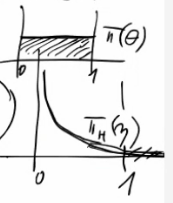
\includegraphics[width=0.25\linewidth]{pictures/P7_1}
		\caption{}
		\label{fig:p71}
	\end{figure}
\end{example}
\begin{example}
	Mějme $X\sim f(x|\t),~\t\in\Theta_j,~\t\sim\pi(\t),~\mathcal{F}=\{f(x|\t)\}$. Víme, že $\eta=\inv{H}(\t)$, tzn. $\t=H(\eta)$. 
	$$ f_H(x|\eta)=f\big(x|\t=H(\eta)\big)=f\big(x|H(\eta)\big)...\mathcal{F}$$
	$$ \pi_H(\eta)=\pi\big(H(\eta)\big)\big|D_H(\eta)\big|$$
	Z ÚBM $\{\mathcal{F},\pi\}$ plyne aposteriorní hustota $\pi(\t|\textbf{x})~\to~\widehat{\t}_B(\textbf{x})=\EE{\pi(\t|\textbf{x})}$. Dále z~ÚBM $\{\mathcal{F},\pi\}$ plyne ÚBM $\{\mathcal{F}_H,\pi_H\}$ a~z~něho aposteriorní hustota $\pi(\eta|\textbf{x})~\to~ \widehat{\eta}_B(\textbf{x})=\EE{\pi(\eta|\textbf{x})}$. 
	
	Pozor na~$\widehat{\t}_B\neq H(\widehat{\eta}_B)$! To může být problém.
\end{example}
\begin{theorem}[Jeffreys]
	Máme ÚBM $\mathcal{F},\pi(\t),~\eta=\inv{H}(\t),~\t=H(\eta)$ a~předpokládejme, že $\t\in\Theta\subset\R^k$ a~že $H$ je regulární transformace. Nechť $\mathcal{F}$ je regulární systém hustot ($\fregp$). $\mathcal{F}_H,\pi_H$. Volme $\pi(\t)=\sqrt{\det \mathbb{J}(\t)}$, kde $\mathbb{J}(\t)$ je FIM pro~$\t$ v~$\mathcal{F}$. Pak $\pi_H(\eta)=\sqrt{\det \mathbb{J}_H(\eta)}$ a~platí, že 
	$$ \int_B\pi(\t|\textbf{x})\d\t=\int_{\inv{H}(B)}\pi_H(\eta|\textbf{x})\d\eta,\qquad\forall B\in\Bb_\Theta.$$
	\begin{proof}
		Pro $k=1$: (zbytek ponecháno čtenáři)\begin{enumerate}[a)]
			\item \[
			\begin{split}
			\int_B\pi(\t|\textbf{x})\d\t&=\frac{1}{c}\int_B f(\textbf{x}|\t)\pi(\t)\d\t=\left|\begin{array}{c}
			\t=H(\eta)\\D_H(\eta)
			\end{array}
			\right|=\frac{1}{c}\int_{\inv{H}(B)}\underbrace{f\big(\textbf{x}|H(\eta)\big)}_{f_H(\eta)}\underbrace{\pi\big(H(\eta)\big)\big|D_H(\eta)\big|}_{\pi_H(\eta)}\d\eta=\\&=\frac{1}{c_{(H)}}\int_{\inv{H}(B)}f_H\pi_H\d\eta=\int_{\inv{H}(B)}\pi(\eta|\textbf{x})\d\eta
			\end{split}
			\]
			\item Protože 
			$$ \mathbb{J}_H(\eta)=\EE{\frac{\partial\log f_H(\eta)}{\partial\eta}}^2=\EE{\frac{\partial\log f(x|H(\eta))}{\partial\t}\frac{\partial H(\eta)}{\partial\eta}}^2=D_H^2(\eta)\mathbb{J}\big(H(\eta)\big) ,$$
			pak \[
			\begin{split}
			\pi_H(\eta)&=\pi\big(H(\eta)\big)\big|D_H(\eta)\big|=\sqrt{\det \mathbb{J}\big(H(\eta)\big)}\cdot\big|D_H(\eta)\big|=\sqrt{\det \mathbb{J}_H(\eta)D_H^{-2}(\eta)}\cdot\big|D_H(\eta)\big|=\\&=\sqrt{\det \mathbb{J}_H(\eta)}
			\end{split}
			\]
			Tedy $\pi(\t)=\sqrt{\det \mathbb{J}(\t)}$, což je \textbf{Jeffraysova apriorní hustota} (často bývá nevlastní).
		\end{enumerate}
	\end{proof}
\end{theorem}
\begin{example}
	Mějme $X\sim f_X(x|\lambda)=\mathrm{Po}(\lambda)$, tzn. $f_{X_j}=\frac{\lambda^{x_j}}{x_j!}\e{-\lambda},~f_\textbf{x}(\textbf{x}|\lambda)=\frac{\lambda^{\sum x_j}}{\prod x_j!}\e{-n\lambda},~\lambda>0$.\begin{enumerate}[a)]
		\item Pokud je $\lambda$ neznámé, pak $\pi(\lambda)=1$ na~$\R^+$ (nevlastní).
		$$
		\pi(\lambda|\textbf{x})=\frac{\fex \pi}{\int_{0}^{+\infty}\fex\pi\d\lambda}=\frac{1}{c}\frac{1}{\prod x_j!}\lambda^{\sumjn x_j}\e{-n\lambda}\sim\mathrm{Gamma}\big(\sumjn x_j+1,n\big).$$
		Bayesovský odhad $$\widehat{\lambda}_B=\EE{\mathrm{Gamma}(\underbrace{\sum x_j+1}_{\alpha},\underbrace{n}_\beta)}=\frac{\alpha}{beta}=\frac{\sumjn x_j}{n}+\frac{1}{n}=\Oxn+\frac{1}{n}\sim \Oxn~(MLE).$$
		\item Jeffrys: $$\pi(\lambda)=\sqrt{\det \mathbb{J}(\lambda)}=\sqrt{\det \EE{-\frac{\partial^2\log\fex}{\partial\lambda^2}}}=\sqrt{n\cdot\frac{1}{\lambda}}=\sqrt{n}\frac{1}{\sqrt{\lambda}}.$$
		Volba $\pi(\lambda)=\frac{1}{\sqrt{\lambda}}$ viz obr. \ref{fig:p72}.
		\begin{figure}[h]
			\centering
			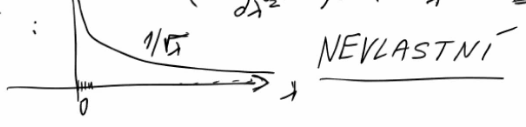
\includegraphics[width=0.5\linewidth]{pictures/P7_2}
			\caption{Nevlastní}
			\label{fig:p72}
		\end{figure}
		$$ \pi(\lambda|\textbf{x})=\frac{f \pi(\lambda)c}{\int f\pi(\lambda)c\d\lambda}=\frac{1}{c'}\lambda^{\sumjn x_j-\frac{1}{2}}\e{-n\lambda}\sim\mathrm{Gamma}\Big(\underbrace{\sumjn x_j+\frac{1}{2}}_{\tilde{\alpha}},\underbrace{n}_{\tilde{\beta}}\Big).$$
		Bayes $\widehat{\lambda}_B^J=\EE{\mathrm{Gamma}(\tilde{\alpha},\tilde{\beta})}=\frac{\alpha}{\beta}=\Oxn+\frac{1}{2n}\sim\Oxn$ (MLE, velká $n$).
	\end{enumerate}
	Pro $n$ malé je volba a) nebo b) vlivná.
\end{example}

\section{Limitní aposteriorní hustoty ($\widehat{\t}_B$)}
Mějme ÚBM $\{\mathcal{F},\pi(\t)\}$ a~předpokládejme, že $\pi\in\Pi=\{\pi(\t),\boldsymbol{\lambda}:\boldsymbol{\lambda}\in\Lambda\}=\mathcal{H}$. Volme $\lambda_0\in\partial\Lambda$ hranice a~definujme $\pi_{\lambda_0}(\t)=\lim\limits_{\lambda\to\lambda_0}c\cdot \pi(\t,\lambda)$, která bývá nevlastní. 

Dále pak (s použitím záměny integrálu a~limity) $$\pi_{\lambda_0}(\t|\textbf{x})\equal{ozn}\frac{f\pi_{\lambda_0}(\t)}{\int_\Theta f\pi_{\lambda_0}(\t)\d\t}=\frac{f\lim\limits_{\lambda\to\lambda_0}c\pi(\t,\lambda)}{\int_\Theta f\lim\limits_{\lambda\to\lambda_0}c\pi(\t,\lambda) \d\t}=\lim\limits_{\substack{
		\lambda\to\lambda_0\in\partial\Lambda\\\lambda\in\Lambda	}
}\frac{f\pi(\t,\lambda)}{\int f\pi(\t,\lambda)\d\t}=\lim\limits_{\lambda\to\lambda_0}\pi(\t|\textbf{x},\lambda).$$
Z toho vyplývá, že $\htb^\mathrm{lim} =\EE{\pi_{\lambda_0}(\t|\textbf{x})}$, což často vede na~klasickou statistickou proceduru.

\begin{example}
	Mějme $X\sim f_X=\mathrm{Exp}(\t),~f_X=\theta\e{-\t x},~\t>0$, $$\mathcal{H}=\{\t\sim\mathrm{Gamma}(\alpha,\beta),~\text{tzn. }\pi\big(\t,\underbrace{(\alpha,\beta)}_{\boldsymbol{\lambda}}\big)=\t^{\alpha-1}\e{-\beta\t}\},~\Lambda=\R^{2+}.$$ $\boldsymbol{\lambda}_0=(0,0)\in\partial\Lambda\Rightarrow\pi_{0,0}(\t)=\lim\limits_{(\alpha,\beta)\to(0,0_+)}\t^{\alpha-1}\e{-\beta\t}=\frac{1}{\t}$ (nevlastní).
	$$\pi_{(0,0)}(\t|\textbf{x})=\frac{f\cdot\frac{1}{\t}}{\int_{0}^{+\infty}f\cdot\frac{1}{\t}\d\t}\equal{iid}\frac{\t^n\e{-\t\sumjn x_j}\cdot\frac{1}{\t}}{c}=\t^{n-1}\e{-\t\sumjn x_j}\sim\mathrm{Gamma}\Big(n,\sumjn x_j\Big),$$
	$$\htb^{\mathrm{lim}}=\E\Big[\mathrm{Gamma}\Big(n,\sumjn x_j\Big)\Big]=\frac{n}{\sumjn x_j}=\inv{(\Oxn)}=\html.$$
\end{example}
\begin{example}
	Volba $\pi(\t)$? Subjektivní. New England Your. of Medicine - studie\begin{enumerate}[1)]
		\item léčba rakoviny plic - operace - víme, že šance na~přežití je 68\%, ale jen 44\% lidí by tam šla. 
		\item léčba rakoviny plic - operace - víme, že pravděpodobnost úmrtí je 32\%, ale jen 18\% lidí by tam šla. 
	\end{enumerate}
\end{example}

\subsection{Empirical Bayes}
Máme $\mathcal{H}=\{\pi(\t,\lambda):\lambda\in\Lambda\}$. Spočítá se~$m_\lambda(\textbf{x})=\int_\Theta\underbrace{f(\textbf{x}|\t)\pi(\t,\lambda)}_{\phi(\textbf{x},\t,\lambda)}\d\t$. Data $\textbf{X}..\textbf{x}$ na~základě dat odhadneme $\widehat{\lambda}(\textbf{x})$ v~té $m_\lambda(\textbf{x})$ a~provedeme BP s~apriorní hustotou $\pi(\t,\widehat{\lambda}_{\mathrm{ML}})$ klasickou statistickou procedurou $\widehat{\lambda}_{\mathrm{ML}}$.

Principem ME $H(\pi)=-\int_\Theta\pi(\t)\log \pi(\t)\d\t$ .. $\pi$ volíme tak, aby $H(\pi)$ bylo maximální.

\chapter{Bayesovský princip, bayesovský úplný model, výhody jeho použití, vztah k~ostatním principům.}


\chapter{Třídy optimálních strategii, užitková funkce a~podmínky pro~existenci užitkové funkce.}


\chapter{Bayesovské riziko, aposteriorní hustota, prediktivní bayesovská hustota.}


\chapter{Asymptotické vlastnosti aposteriorní hustoty a~bayesovských bodových odhadů.}


\chapter{Formy apriorní informace, princip neurčitosti, Jeffreysova hustota, ukázky.}


\chapter{Konjugované systémy apriorních hustot, princip maximální entropie, limitní aposteriorní hustoty, příklady.}


\chapter{Nejméně příznivá apriorní rozdělení, souvislost s~minimaxním principem rozhodování.}


\chapter{Přípustnost bayesovského řešení, Steinův efekt pro~sféricky symetrická rozdělení, Bergerův jev.}


\chapter{Grupy transformací, ekvivariantní odhady a~jejich bayesovská representace.}


\chapter{Bayesovské odhady pro~absolutní, multi-lineární, (váženou) kvadratickou a~0-1 ztrátovou funkci.}


%\chapter{Hierarchický bayesovský model, empirický Bayes a~jeho suboptimalita, aplikace.}


\chapter{Laplaceova asymptotická expanze, podmínky regularity stochastické aproximace, numerické kvadratury.}


%\chapter{Vzorkování podle důležitosti, Metropolisův algoritmus, variační Bayes.} - prý se nestihlo


\chapter{Bayesovská strategie testování hypotéz, Bayes faktor, vlastnosti, porovnání s~klasickými testy.}




%


% ****************************************************************************************************************************
%                             BACKMATTER
% ****************************************************************************************************************************
\backmatter
%\input{literatura}
\printindex

\end{document}
